\begin{enumerate}[label=\thechapter.\arabic*,ref=\thechapter.\theenumi]

\item Consider the differential equation $\frac{d^2y}{dx^2}-2\frac{dy}{dx}+y=0$. The boundary conditions are $y=0$ and $\frac{dy}{dx}=1$ at $x=0$. Then the value of $y$ at $x=\frac{1}{2}$ \hfill (GATE AE 2022)\\
\solution
\input{2022/AE/37/ae_37.tex}
\pagebreak

\item  A process described by the transfer function
\begin{align}
    G_p(s) = \frac{\brak{10s+1}}{\brak{5s+1}} \nonumber
\end{align}
is forced by a unit step input at time $t = 0$. The output value immediately after the unit step input (at $t = 0^+$) is ? \hfill(Gate 2022 CH 34)\\
\solution
\iffalse
\documentclass[journal,12pt,twocolumn]{IEEEtran}
\usepackage{cite}
\usepackage{amsmath,amssymb,amsfonts,amsthm}
\usepackage{algorithmic}
\usepackage{graphicx}
\usepackage{textcomp}
\usepackage{xcolor}
\usepackage{txfonts}
\usepackage{listings}
\usepackage{enumitem}
\usepackage{mathtools}
\usepackage{gensymb}
\usepackage{comment}
\usepackage[breaklinks=true]{hyperref}
\usepackage{tkz-euclide}
\usepackage{listings}
\usepackage{gvv}
\def\inputGnumericTable{}
\usepackage[latin1]{inputenc}
\usepackage{color}
\usepackage{array}
\usepackage{longtable}
\usepackage{calc}
\usepackage{multirow}
\usepackage{hhline}
\usepackage{ifthen}
\usepackage{lscape}
\usepackage{caption}

\newtheorem{theorem}{Theorem}[section]
\newtheorem{problem}{Problem}
\newtheorem{proposition}{Proposition}[section]
\newtheorem{lemma}{Lemma}[section]
\newtheorem{corollary}[theorem]{Corollary}
\newtheorem{example}{Example}[section]
\newtheorem{definition}[problem]{Definition}
\newcommand{\BEQA}{\begin{eqnarray}}
\newcommand{\EEQA}{\end{eqnarray}}
\newcommand{\define}{\stackrel{\triangle}{=}}
\theoremstyle{remark}
\newtheorem{rem}{Remark}
\begin{document}

\bibliographystyle{IEEEtran}
\vspace{3cm}

\title{GATE: CH - 34.2022}
\author{EE23BTECH11010 - Venkatesh D Bandawar $^{*}$% <-this % stops a space
}
\maketitle
% \newpage
\bigskip

% \renewcommand{\thefigure}{\theenumi}
% \renewcommand{\thetable}{\theenumi}

\textbf{Question:} A process described by the transfer function
\begin{align}
    G_p(s) = \frac{\brak{10s+1}}{\brak{5s+1}} \nonumber
\end{align}
is forced by a unit step input at time $t = 0$. The output value immediately after the unit step input (at $t = 0^+$) is ? \hfill(Gate 2022 CH 34)\\
\solution
\fi
\begin{table}[!h] 
\centering
\begin{tabular}{|c|c|}
\hline
     \textbf{Parameters}&\textbf{Description}  \\
     \hline
     $X(s)$ & Laplace transform of $x(t)$ \\
     \hline
     $Y(s)$ & Laplace transform of $y(t)$ \\
     \hline
     $G_p(s) = \frac{Y(s)}{X(s)}$ & Transfer function\\
     \hline
     $x(t) = u(t)$ & unit step function\\
     \hline
\end{tabular}

\caption{Given parameters}
\label{given parameters list.gate.2022.ch.34}
\end{table}
\begin{align}
    G_p(s) = \frac{Y(s)}{X(s)} &= \frac{\brak{10s+1}}{\brak{5s+1}}\\
    u(t) \system{\mathcal{L}} \frac{1}{s} \label{laplace transform of unit function 2022.ch.34}
\end{align}
From equation \eqref{laplace transform of unit function 2022.ch.34}:
\begin{align}
    Y(s) &= \frac{\brak{10s+1}}{s\brak{5s+1}}\\
    &= \frac{1}{s} + \frac{5}{5s+1}
\end{align}
Taking inverse laplace transformation, 
\begin{align}
    \frac{1}{s} &\mathrel{\substack{\mathcal{L}^{-1}\\\longleftrightarrow}} u(t)\\
    \frac{1}{s-c} &\mathrel{\substack{\mathcal{L}^{-1}\\\longleftrightarrow}} e^{ct} u(t)
\end{align}
\begin{align}
    y(t) &= \brak{1 + e^{\frac{-t}{5}}}u(t)\\
    y(0^+) &= 2
\end{align}

\begin{figure}[!h] 
    \centering
    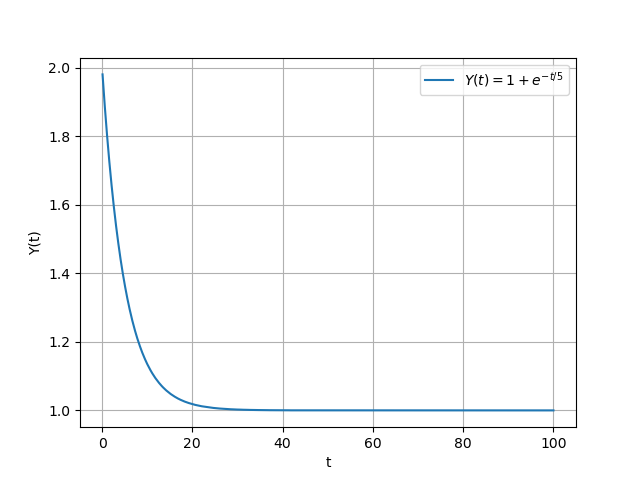
\includegraphics[width=\columnwidth]{2022/CH/34/figs/Graph_of_y(t).png}
    \caption{Graph of y(t)}
    \label{fig:Graph1_gate_CE_30}
    \end{figure}


\pagebreak
\item The transfer function of a real system $H(S)$ is given as:
\begin{align}
    H(s) = \frac{As + B}{s^2 + Cs + D}\nonumber
\end{align}
where $A, B, C$ and $D$ are positive constants. This system cannot operate as
\begin{enumerate}[label={(\Alph*)}]
    \item Low pass filter
    \item High pass filter
    \item Band pass filter
    \item An Integrator
\end{enumerate}\hfill(GATE EE 11 2022)

\solution
 \iffalse
\let\negmedspace\undefined
\let\negthickspace\undefined
\documentclass[journal,12pt,twocolumn]{IEEEtran}
\usepackage{cite}
\usepackage{amsmath,amssymb,amsfonts,amsthm}
\usepackage{algorithmic}
\usepackage{graphicx}
\usepackage{textcomp}
\usepackage{xcolor}
\usepackage{txfonts}
\usepackage{listings}
\usepackage{enumitem}
\usepackage{mathtools}
\usepackage{gensymb}
\usepackage{comment}
\usepackage[breaklinks=true]{hyperref}
\usepackage{tkz-euclide} 
\usepackage{listings}
\usepackage{gvv} 
\usepackage{caption}
\def\inputGnumericTable{}                   

%\usepackage[latin1]{inputenc}                                
\usepackage{color}                                            
\usepackage{array}                                            
\usepackage{longtable}                                       
\usepackage{calc}                                             
\usepackage{multirow}                                         
\usepackage{hhline}                                           
\usepackage{ifthen}                                           
\usepackage{lscape}
\usepackage{tikz}
\newtheorem{theorem}{Theorem}[section]
\newtheorem{problem}{Problem}
\newtheorem{proposition}{Proposition}[section]
\newtheorem{lemma}{Lemma}[section]
\newtheorem{corollary}[theorem]{Corollary}
\newtheorem{example}{Example}[section]
\newtheorem{definition}[problem]{Definition}
\newcommand{\BEQA}{\begin{eqnarray}}
\newcommand{\EEQA}{\end{eqnarray}}
\newcommand{\define}{\stackrel{\triangle}{=}}
\theoremstyle{remark}
\newtheorem{rem}{Remark}

\begin{document}

\bibliographystyle{IEEEtran}
\vspace{3cm}

\title{GATE: EE - 11.2022}
\author{EE23BTECH11013 - Avyaaz$^{*}$% <-this % stops a space 
}
\maketitle
\newpage
\bigskip

\renewcommand{\thefigure}{\arabic{figure}}
\renewcommand{\thetable}{\arabic{table}}

\large\textbf{\textsl{Question:}}
The transfer function of a real system $H(S)$ is given as:
\begin{align}
    H(s) = \frac{As + B}{s^2 + Cs + D}\nonumber
\end{align}
where $A, B, C$ and $D$ are positive constants. This system cannot operate as
\begin{enumerate}[label={(\Alph*)}]
    \item Low pass filter
    \item High pass filter
    \item Band pass filter
    \item An Integrator
\end{enumerate}\hfill(GATE EE 11 2022) \\
\solution
\fi
The transfer function $H(s)$ is given by: 
\begin{align}
    H(s) = \frac{As + B}{s^2 + Cs + D}\label{eq:given.EE.11.2022}
\end{align}
Put $s = j\omega$ in \eqref{eq:given.EE.11.2022}:
\begin{align}
    H(j\omega) = \frac{A(j\omega) + B}{(j\omega)^2 + C(j\omega) + D} \\
    |H(j\omega)| = \frac{\sqrt{(A\omega)^2 + B^2}}{\sqrt{(D - \omega^2)^2 + (\omega C)^2}}\label{eq:magnitude.EE.11.2022}
\end{align}


\begin{table}[htbp]
\setlength{\extrarowheight}{4pt}
\setlength{\tabcolsep}{3pt}
\centering
\begin{tabular}{|c|c|}
\hline
\textbf{Parameter} & \textbf{Description}\\
\hline 
Low Pass Filter & The gain should be finite at low frequency  \\
\hline
High Pass Filter &The gain should be finite at high frequency \\
\hline
Band Pass Filter& Finite gain over frequency band \\
\hline
Integrator & Transfer function should have at least\\& one pole at origin \\
\hline
\end{tabular}

\caption{Conditions}
\label{tab:inputs.EE.11.2022}
\end{table}
% \item \noindent From \tabref{tab:inputs.EE.11.2022} and equation \eqref{eq:magnitude.EE.11.2022}:
\begin{enumerate}[label={\alph*)}]
    \item Low Pass Filter:
    
  At low frequency $(\omega = 0 )$:
 \begin{align}
     |H(\omega = 0)| = \frac{B}{D}\label{eq:lowpass.EE.11.2022}
 \end{align}
$\therefore$ H(s) can operate as Low pass filter.

\item High Pass Filter:

% From \tabref{tab:inputs.EE.11.2022} and equation \eqref{eq:magnitude.EE.11.2022}:

At high frequency $(\omega = \infty )$:
 \begin{align}
     |H(\omega = \infty)| = 0 \label{eq:highpass.EE.11.2022}
 \end{align}
 % From \tabref{tab:inputs.EE.11.2022}:
 
$\therefore$ $H(s)$ cannot operate as High pass filter.
\item Band Pass Filter:

 Assuming B is a very less positive valued constant as compared to others:
\begin{align}
        |H(j\omega)| = \frac{(A\omega)}{\sqrt{(D - \omega^2)^2 + (\omega C)^2}}\\
   \implies      |H(\omega = 0)| = 0 \text{ and }  |H(\omega = \infty)| = 0 \label{eq:bandpass.EE.11.2022}
\end{align}

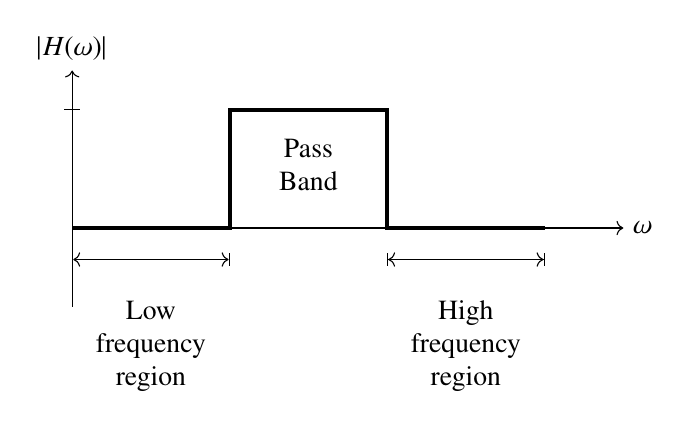
\begin{tikzpicture}
  
    \draw[->] (0,0) -- (7,0) node[right] {$\omega$};
   
    \draw[->] (0,-1) -- (0,2) node[above] {$|H(\omega)|$};
  
    \draw[line width=1.5pt]  (0,0) -- (2,0) -- (2,1.5) -- (4,1.5) -- (4,0) --(6,0);
    \draw[-]{(0,1.5)};
      \draw (-0.1,1.5) -- (0.1,1.5);
         \draw[|<->|]{(0,-0.4) -- (2,-0.4)};
    \node[align=center] at (1,-1.5) {Low \\frequency\\ region};
         \draw[| <-> |]{(4,-0.4) -- (6,-0.4)};
    \node[align=center] at (5,-1.5) {High \\frequency\\ region};
    \node[align=center] at (3,0.8) {Pass\\Band};

\end{tikzpicture}
$\because$ $H(s)$ passes frequency between low and high frequencies.

$\therefore$ $H(s)$ can operate as a band pass filter.
\item Integrator:

At very high value of frequency$(\omega\mkern-4mu \rightarrow\mkern-6mu\infty)$:
\begin{align}
    H(s) \approx \frac{As}{s^2} \approx \frac{A}{s}\label{eq:integrator.EE.11.2022}
\end{align}
From \tabref{tab:inputs.EE.11.2022}:

$\therefore$ $H(s)$ can operate as an Integrator.
\end{enumerate}
% From equations \eqref{eq:lowpass.EE.11.2022},\eqref{eq:highpass.EE.11.2022},\eqref{eq:bandpass.EE.11.2022} and \eqref{eq:integrator.EE.11.2022}:

% The Transfer function $H(s)$ cannot be operated as a High pass filter.
% \begin{figure}[htbp]
%     \centering
%     \includegraphics[width = \columnwidth]{}
%   \caption{}
%     \label{fig:graph1}
% \end{figure}

% \bibliographystyle{IEEEtran}
%\end{document}

\pagebreak

\item In a circuit, there is a series connection of an ideal resistor and an ideal capacitor.
The conduction current (in Amperes) through the resistor is $2\sin\brak{t + \frac{\pi}{2}}$. The displacement current (in Amperes) through the capacitor is \rule{1cm}{0.15mm}.\\ 
\begin{enumerate}[label=(\Alph*)]
    \item $2\sin\brak{t}$
    \item $2\sin\brak{t+\pi}$
    \item $2\sin\brak{t +\frac{\pi}{2}}$
    \item $0$
\end{enumerate}
\hfill(GATE 2022 EC 24)\\
\solution
\iffalse
\documentclass[journal,12pt,twocolumn]{IEEEtran}
\usepackage{amsmath,amssymb,amsfonts,amsthm}
\usepackage{txfonts}
\usepackage{tkz-euclide}
\usepackage{listings}
\usepackage{gvv}
\usepackage[latin1]{inputenc}
\usepackage{adjustbox}
\usepackage{array}
\usepackage{tabularx}
\usepackage{enumitem}
\usepackage{pgf}
\usepackage{lmodern}
\usepackage{circuitikz}
\usepackage{tikz}
\usepackage{graphicx}


\begin{document}
\bibliographystyle{IEEEtran}

\vspace{3cm}

\title{}
\author{EE23BTECH11054 -  Sai Krishna Shanigarapu$^{*}$
}
\maketitle
\newpage
\bigskip

% \renewcommand{\thefigure}{\theenumi}
% \renewcommand{\thetable}{\theenumi}

\section*{Gate EC 2022}
54. \hspace{2pt}In a circuit, there is a series connection of an ideal resistor and an ideal capacitor.
The conduction current (in Amperes) through the resistor is $2\sin\brak{t + \frac{\pi}{2}}$. The displacement current (in Amperes) through the capacitor is \rule{1cm}{0.15mm}.\\ 
\begin{enumerate}[label=(\Alph*)]
    \item $2\sin\brak{t}$
    \item $2\sin\brak{t+\pi}$
    \item $2\sin\brak{t +\frac{\pi}{2}}$
    \item $0$
\end{enumerate}
\hfill(GATE EC 2022)

\solution
\fi
\begin{table}[ht]
       \setlength{\arrayrulewidth}{0.3mm}
\setlength{\tabcolsep}{20pt}
\renewcommand{\arraystretch}{1.5}

\begin{tabular}{|c|c|c|}
\hline
Parameter& Description & Value\\
\hline
$I_c$ & Conduction Current & $2\sin\brak{t + \frac{\pi}{2}}$\\
\hline
%$I_d$ & Displacement current & ?\\
%\hline
$A$ & Cross-sectional area & \\
\hline
\end{tabular}

    \caption{Parameters}
    \label{tab:tab_gate_ec_2022_24_1}
\end{table}


\begin{table}[ht]
       \setlength{\arrayrulewidth}{0.3mm}
\setlength{\tabcolsep}{20pt}
\renewcommand{\arraystretch}{1.5}

\begin{tabular}{|c|c|c|}
\hline
Parameter & Description & Formula\\
\hline
$Q$ & Charge & $\int I_c\, dt$\\
\hline
$D$ & Electric Displacement & $\frac{Q}{A}$\\ 
\hline
$J_D$ & Displacement current density & $\frac{\partial D}{\partial t}$\\
\hline
$I_D$ & Displacement current & $J_D\text{ x }A$\\
\hline




\end{tabular}

    \caption{Formulae}
    \label{tab:tab_gate_ec_2022_24_2}
\end{table}

\begin{table}[ht]
       \setlength{\arrayrulewidth}{0.3mm}
\setlength{\tabcolsep}{20pt}
\renewcommand{\arraystretch}{1.5}



\begin{tabular}{|c|c|}
\hline

S Domain & Time Domain\\
\hline
$\frac{1}{s}$ & $u\brak{t}$\\
\hline
$\frac{-s}{a^2+s^2}$ & $-\cos\brak{at}$\\
\hline
$\frac{a}{a^2+s^2}$ & $\sin\brak{at}$\\
\hline
$\frac{1}{s+a}$ & $e^{-at}$\\
\hline

\end{tabular}


    \caption{Laplace transforms}
    \label{tab:tab_gate_ec_2022_24_3}
\end{table}

\begin{align}
    \mathcal{L}\sbrak{\int f\brak{t}\, dt} &= \int_{0}^{\infty}\sbrak{\int f\brak{t}\, dt}e^{-st}\, dt\\
    &= \int_{0}^{\infty}u\, dv \quad \text{where}\begin{cases}
  u =\int f\brak{t}dt \\
  dv  =e^{-st}dt
\end{cases}\\
&= uv - v\int du\\
&= \frac{1}{s}\int f\brak{t}dt|_0 + \frac{1}{s}\int_{0}^{\infty}f\brak{t}e^{-st}dt\\
&\implies \frac{1}{s}\int f\brak{t}dt|_0 + \frac{1}{s}F\brak{s} \label{eq:eq_gate_ec_2022_24_1}
\end{align}


\begin{figure}[ht]
  \centering
      \begin{circuitikz}[american]
\draw (0,3) to [short,*-, i=$i_c$] (1,3) to [R=$R$] (4,3);
\draw (0,0) to [short, *-] (4,0);
\draw (4,3) to [short, i=$i_d$] (4,2.5) to [C=$C$] (4,0);
\end{circuitikz}
  \caption{Circuit 1}
\end{figure}

From Table \ref{tab:tab_gate_ec_2022_24_2}, Table \ref{tab:tab_gate_ec_2022_24_3} and eq (\ref{eq:eq_gate_ec_2022_24_1})
\begin{align}
    I_c\brak{s} &= \frac{2s}{s^2 + 1}\\
    Q_c\brak{s} &= \frac{2}{s\brak{s^2 + 1}}\\
    D\brak{s} &= \frac{1}{A}\brak{\frac{2}{s\brak{s^2 + 1}}}\\
    J_D\brak{s} &= \frac{2}{A}\brak{\frac{1}{s^2 + 1}}\\
    I_D\brak{s} &= \frac{2}{s^2 + 1}\\
    \implies I_D &= 2\sin{t}
\end{align}


\begin{figure}[ht]
  \centering
      \begin{tikzpicture}

        \draw[->] (-0.5,0) -- (4.5,0) node[right]{$E_{\text{ref}}$};
        \draw[->] (0,-0.5) -- (0,4.5) node[above]{$J_d$};
        

        \draw (0,0) -- (4,4);
        

        \draw[dashed] (4,0) -- (4,4);
        \node[right] at (4,4) {$\overline{J}$};
        \draw[dotted] (4,4) -- (4,0) node[below]{$J_c$};

        \draw[dashed] (0,4) -- (4,4);
        \draw[dotted] (4,4) -- (0,4) node[left]{$J_d$};
        

        \draw[->] (0.5,0) arc (0:90:0.5);
        \node[right] at (0.5,0.3) {$\frac{\pi}{2}$};
\end{tikzpicture}


  \caption{Phasor plot}
  \label{fig:fig_gate_ec_2022_24_1}
\end{figure}

From figure \ref{fig:fig_gate_ec_2022_24_1}, phase of $I_d$ is $\frac{\pi}{2}$

\begin{align}
    \therefore I_d = 2\sin\brak{t + \frac{\pi}{2}}
\end{align}
$\therefore$ (C) is correct.


\begin{figure}[ht]
    \centering
    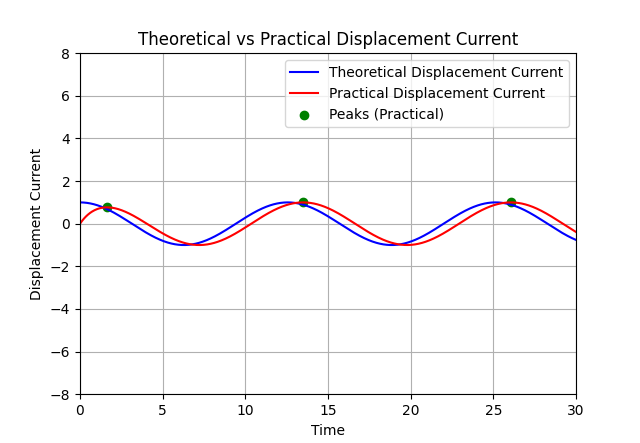
\includegraphics[width=\columnwidth]{2022/EC/24/figs/Figure_2.png}
    \caption{Thoritical vs Practical simulation}
    \label{fig:fig_gate_ec_2022_24_2}
\end{figure}

\begin{figure}[ht]
    \centering
    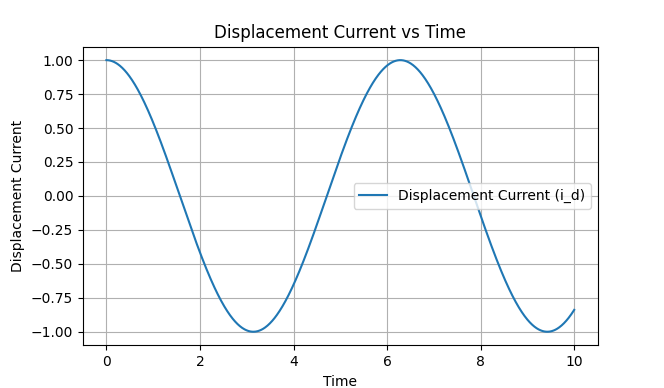
\includegraphics[width=\columnwidth]{2022/EC/24/figs/Figure_4.png}
    \caption{Displacement current}
    \label{fig:fig_gate_ec_2022_24_3}
\end{figure}



%\end{document}

\newpage

\item Given, $y=f\brak{x}$; $\frac{d^2y}{dx2}+4y=0; y\brak{0}=0; \frac{dy}{dx}\brak{0}=1$. The problem is a/an \\
\begin{enumerate}[label=(\alph*)]
    \item initial value problem having soluition $y=x$
    \item boundary value problem having soluition $y=x$
    \item initial value problem having soluition $y=\frac{1}{2}\sin 2x$
    \item boundary value problem having soluition {$y=\frac{1}{2}\sin 2x$}
\end{enumerate} \hfill(GATE 2022 ES)    \\
\solution
\iffalse
\let\negmedspace\undefined
\let\negthickspace\undefined
\documentclass[journal,12pt,twocolumn]{IEEEtran}
\usepackage{cite}
\usepackage{amsmath,amssymb,amsfonts,amsthm}
\usepackage{algorithmic}
\usepackage{graphicx}
\usepackage{textcomp}
\usepackage{xcolor}
\usepackage{txfonts}
\usepackage{listings}
\usepackage{enumitem}
\usepackage{mathtools}
\usepackage{gensymb}
\usepackage{comment}
\usepackage[breaklinks=true]{hyperref}
\usepackage{tkz-euclide} 
\usepackage{listings}
\usepackage{gvv}                                        
\def\inputGnumericTable{}                                 
\usepackage[latin1]{inputenc}                                
\usepackage{color}                                            
\usepackage{array}                                            
\usepackage{longtable}                                       
\usepackage{calc}                                             
\usepackage{multirow}                                         
\usepackage{hhline}                                           
\usepackage{ifthen}                                           
\usepackage{lscape}

\newtheorem{theorem}{Theorem}[section]
\newtheorem{problem}{Problem}
\newtheorem{proposition}{Proposition}[section]
\newtheorem{lemma}{Lemma}[section]
\newtheorem{corollary}[theorem]{Corollary}
\newtheorem{example}{Example}[section]
\newtheorem{definition}[problem]{Definition}
\newcommand{\BEQA}{\begin{eqnarray}}
\newcommand{\EEQA}{\end{eqnarray}}
\newcommand{\define}{\stackrel{\triangle}{=}}
\theoremstyle{remark}
\newtheorem{rem}{Remark}
\begin{document}
\parindent 0px
\bibliographystyle{IEEEtran}
\title{GATE: ES - 36.2022}
\author{EE22BTECH11219 - Rada Sai Sujan$^{}$% <-this % stops a space
}
\maketitle
\newpage
\bigskip
\section*{Question}
Given, $y=f\brak{x}$; $\frac{d^2y}{dx2}+4y=0; y\brak{0}=0; \frac{dy}{dx}\brak{0}=1$. The problem is a/an \\
\begin{enumerate}[label=(\alph*)]
    \item initial value problem having soluition $y=x$
    \item boundary value problem having soluition $y=x$
    \item initial value problem having soluition $y=\frac{1}{2}\sin 2x$
    \item boundary value problem having soluition {$y=\frac{1}{2}\sin 2x$}
\end{enumerate} \hfill(GATE 2022 ES)    \\
\solution
\fi

The above equation can be written as,
\begin{align}
    y^{\prime\prime}\brak{t}+4y\brak{t}=0
\end{align}
Using the Laplace transformation pairs,
\begin{align}
    y^{\prime\prime}\brak{t} &\overset{\mathcal{L}}{ \longleftrightarrow} s^2Y\brak{s}-sy\brak{0}-y^{\prime}\brak{0}    \\
    y\brak{t} &\overset{\mathcal{L}}{ \longleftrightarrow} Y\brak{s}    \\
    \sin at &\overset{\mathcal{L}}{ \longleftrightarrow} \frac{a}{a^2+s^2}  \label{equation:gate.es.2022.4}
\end{align}
Applying Laplace transform for the equation we get,
\begin{align}
    s^2Y\brak{s}-1+4Y\brak{s} &= 0  \\
    \implies Y\brak{s} &= \frac{1}{4+s^2}
\end{align}
Now, applying inverse laplace transform we get,
\begin{align}
    y\brak{t} &= \frac{1}{2}\sin 2t \quad \text{(from \eqref{equation:gate.es.2022.4})}
\end{align}
Since, the conditions at the same point\brak{0} are mentioned, it is an initial valued problem having solution $y=\frac{1}{2}\sin 2x$.
\begin{figure}[ht]
    \centering
    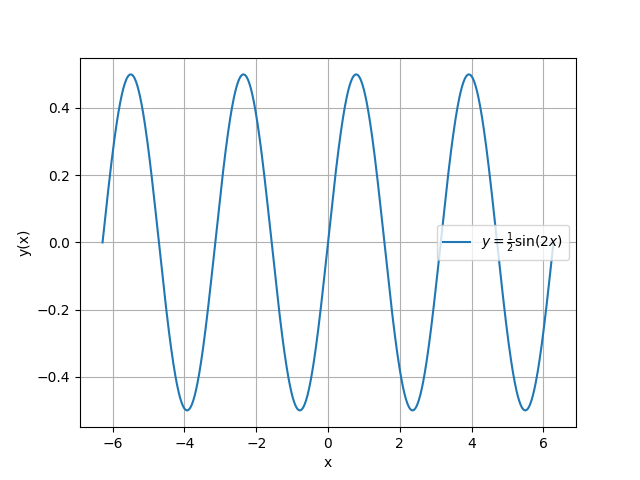
\includegraphics[width=\columnwidth]{2022/ES/36/figs/a.png}
    \caption{$y\brak{x}$ $vs$ $x$ graph}
    \label{figure:gate.2022.es.36Q.1}
\end{figure}

\newpage
\item Let a causal LTI system be governed by the following differential equation, 
\begin{align}
    y\brak{t} + \frac{1}{4}\frac{dy}{dt} = 2x\brak{t} \label{eq1}
\end{align}
where $x\brak{t}$ and $y\brak{t}$ are the input and output respectively. It's impulse response is 
\hfill (GATE EE-2022)\\
\solution
\iffalse
\let\negmedspace\undefined
\let\negthickspace\undefined
\documentclass[journal,12pt,twocolumn]{IEEEtran}
\usepackage{cite}
\usepackage{amsmath,amssymb,amsfonts,amsthm}
\usepackage{algorithmic}
\usepackage{graphicx}
\usepackage{textcomp}
\usepackage{xcolor}
\usepackage{txfonts}
\usepackage{listings}
\usepackage{enumitem}
\usepackage{mathtools}
\usepackage{gensymb}
\usepackage{comment}
\usepackage[breaklinks=true]{hyperref}
\usepackage{tkz-euclide} 
\usepackage{listings}
\usepackage{gvv}                                        
\def\inputGnumericTable{}                                 
\usepackage[latin1]{inputenc}                                
\usepackage{color}                                            
\newtheorem{theorem}{Theorem}[section]
\usepackage{array}                                            
\usepackage{longtable}                                       
\usepackage{calc}                                             
\usepackage{multirow}                                         
\usepackage{hhline}                                           
\usepackage{ifthen}                                           
\usepackage{lscape}
\newtheorem{problem}{Problem}
\newtheorem{proposition}{Proposition}[section]
\newtheorem{lemma}{Lemma}[section]
\newtheorem{corollary}[theorem]{Corollary}
\newtheorem{example}{Example}[section]
\newtheorem{definition}[problem]{Definition}
\newcommand{\BEQA}{\begin{eqnarray}}
\newcommand{\EEQA}{\end{eqnarray}}
\newcommand{\define}{\stackrel{\triangle}{=}}
\theoremstyle{remark}
\newtheorem{rem}{Remark}
\begin{document}
\bibliographystyle{IEEEtran}
\vspace{3cm}
\title{GATE 22 EE/46}
\author{EE23BTECH11040 - Manoj Kumar Ambatipudi$^{*}$% <-this % stops a space
}
\maketitle
\newpage
\bigskip
\renewcommand{\thefigure}{\theenumi}
\renewcommand{\thetable}{\theenumi}
\textbf{QUESTION:}
Let a causal LTI system be governed by the following differential equation, 
\begin{align}
    y\brak{t} + \frac{1}{4}\frac{dy}{dt} = 2x\brak{t} \label{eq1}
\end{align}
where $x\brak{t}$ and $y\brak{t}$ are the input and output respectively. It's impulse response is 
\hfill (GATE EE-2022)\\
\fi
\textbf{Solution:}

From \eqref{eq1}, corresponding Laplace transform, 
\begin{align}
    Y\brak{s} + \frac{1}{4}\brak{sY\brak{s} - y\brak{0}} = 2X\brak{s}
\end{align}
Since it is causal LTI system, 
\begin{align}
    y\brak{0} &= 0\\
	\implies Y\brak{s} + \frac{1}{4}sY\brak{s} &= 2X\brak{s}\\
    \implies Y\brak{s} &= X\brak{s}\frac{8}{4 + s}\\
    \implies H\brak{s} &= \frac{8}{4 + s}\quad ROC:Re\brak{s} > -4
\end{align}
Taking inverse laplace transform and applying causality conditions 
\begin{align}
    h\brak{t} = 8e^{-4t}u\brak{t}
\end{align}
\begin{figure}[h]
\renewcommand\thefigure{1}
    \centering
    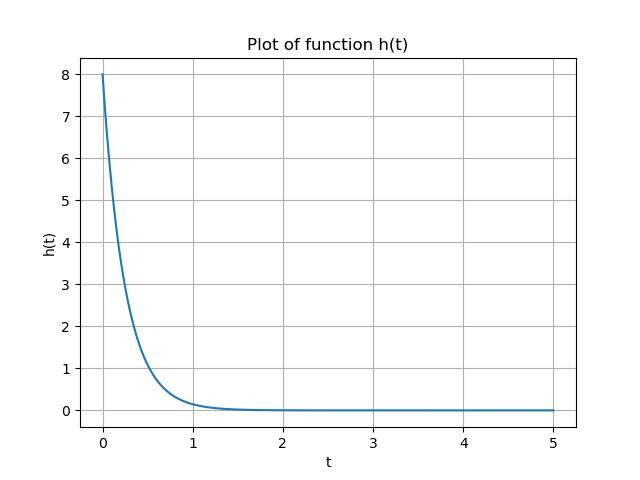
\includegraphics[width=1.0\columnwidth]{2022/EE/46/figs/fig_1.jpg}
    \caption{Plot of $h\brak{n}$, taken from python3}
    \label{fig:enter-label}
\end{figure}


\item Assuming $s>0$; Laplace transform for $f\brak{x} = sin\brak{ax}$ is
\begin{enumerate}[label=(\Alph*)]
    \item $\frac{a}{s^2+a^2}$
    \item $\frac{s}{s^2+a^2}$
    \item $\frac{a}{s^2-a^2}$
    \item $\frac{s}{s^2-a^2}$
\end{enumerate} \hfill(GATE 2022 ES)\\
\solution
\iffalse
\let\negmedspace\undefined
\let\negthickspace\undefined
\documentclass[journal,12pt,twocolumn]{IEEEtran}
\usepackage{cite}
\usepackage{amsmath,amssymb,amsfonts,amsthm}
\usepackage{algorithmic}
\usepackage{graphicx}
\usepackage{textcomp}
\usepackage{xcolor}
\usepackage{txfonts}
\usepackage{listings}
\usepackage{enumitem}
\usepackage{mathtools}
\usepackage{gensymb}
\usepackage{comment}
\usepackage[breaklinks=true]{hyperref}
\usepackage{tkz-euclide} 
\usepackage{listings}
\usepackage{gvv}
\def\inputGnumericTable{}                                 
\usepackage[latin1]{inputenc}                                
\usepackage{color}                                            
\usepackage{array}                                            
\usepackage{longtable}                                       
\usepackage{calc}                                             
\usepackage{multirow}                                         
\usepackage{hhline}                                           
\usepackage{ifthen}                                           
\usepackage{lscape}

\newtheorem{theorem}{Theorem}[section]
\newtheorem{problem}{Problem}
\newtheorem{proposition}{Proposition}[section]
\newtheorem{lemma}{Lemma}[section]
\newtheorem{corollary}[theorem]{Corollary}
\newtheorem{example}{Example}[section]
\newtheorem{definition}[problem]{Definition}
\newcommand{\BEQA}{\begin{eqnarray}}
\newcommand{\EEQA}{\end{eqnarray}}
\newcommand{\define}{\stackrel{\triangle}{=}}
\theoremstyle{remark}
\newtheorem{rem}{Remark}

\begin{document}

\bibliographystyle{IEEEtran}
\vspace{3cm}

\title{GATE ES22 13}
\author{EE23BTECH11043 - BHUVANESH SUNIL NEHETE$^{*}$% <-this % stops a space
}
\maketitle
\newpage
\bigskip

\renewcommand{\thefigure}{\theenumi}
\renewcommand{\thetable}{\theenumi}

\bibliographystyle{IEEEtran}

\textbf{Question:}
Assuming $s>0$; Laplace transform for $f\brak{x} = sin\brak{ax}$ is
\begin{enumerate}[label=(\Alph*)]
    \item $\frac{a}{s^2+a^2}$
    \item $\frac{s}{s^2+a^2}$
    \item $\frac{a}{s^2-a^2}$
    \item $\frac{s}{s^2-a^2}$
\end{enumerate}

\solution
\fi
\begin{align}
\mathcal{L}\brak{f\brak{x}}=\int_{-\infty}^{\infty}e^{-sx}f\brak{x}dx\\
\text{We can write} \quad\sin\brak{ax}=\frac{e^{ax}-e^{-ax}}{2i}\label{13es22eq1}
\end{align}
From \eqref{13es22eq1}
\begin{align}
\mathcal{L}\brak{\sin\brak{ax}}&=\int_{0}^{\infty}e^{-sx}\brak{\frac{e^{iax}-e^{-iax}}{2i}}dx\\
&=\frac{1}{2i}\int_{0}^{\infty}e^{-x\brak{s-ia}}-e^{-x\brak{s+ia}}dx\\
&=\frac{1}{2i}\brak{\frac{e^{-x\brak{s-ia}}}{-\brak{s-ia}}+\frac{e^{-x\brak{s+ia}}}{-\brak{s+ia}}}_{0}^{\infty}\\
&=\frac{1}{2i}\brak{\frac{1}{s-ia}-\frac{1}{s+ia}}\\
&=\frac{a}{s^2+a^2}
\end{align}

So, option \brak{A} is correct.

\newpage

\item The input $x(t)$ to a system is related to its output $y(t)$ as \\ \\
$\dfrac{dy(t)}{dt} + y(t) = 3x(t-3)u(t-3)$\\ \\
Here $u(t)$ represents a unit-step function.\\
The transfer function of this system is 
\begin{enumerate}
\item[(A)] $\frac{e^{-3s}}{s+3}$\\
\item[(B)] $\frac{3e^{-3s}}{s+1}$\\
\item[(C)] $\frac{3e^{-\brak{s/3}}}{s+1}$\\
\item[(D)] $\frac{e^{-\brak{s/3}}}{s+3}$
\end{enumerate}
\hfill{(GATE IN 2022)}\\
\solution
\iffalse
\let\negmedspace\undefined
\let\negthickspace\undefined
\documentclass[journal,12pt,twocolumn]{IEEEtran}
\usepackage{cite}
\usepackage{amsmath,amssymb,amsfonts,amsthm}
\usepackage{algorithmic}
\usepackage{graphicx}
\usepackage{textcomp}
\usepackage{xcolor}
\usepackage{txfonts}
\usepackage{listings}
\usepackage{enumitem}
\usepackage{mathtools}
\usepackage{gensymb}
\usepackage{comment}
\usepackage[breaklinks=true]{hyperref}
\usepackage{tkz-euclide} 
\usepackage{listings}                                   
\def\inputGnumericTable{}                                 
\usepackage[latin1]{inputenc}                                
\usepackage{color}                                            
\usepackage{array}                                            
\usepackage{longtable}                                       
\usepackage{calc}  
\usepackage{circuitikz}                                           
\usepackage{multirow}                                         
\usepackage{hhline}                                           
\usepackage{ifthen}                                           
\usepackage{lscape}
\newtheorem{theorem}{Theorem}[section]
\newtheorem{problem}{Problem}
\newtheorem{proposition}{Proposition}[section]
\newtheorem{lemma}{Lemma}[section]
\newtheorem{corollary}[theorem]{Corollary}
\newtheorem{example}{Example}[section]
\newtheorem{definition}[problem]{Definition}
\newcommand{\BEQA}{\begin{eqnarray}}
\newcommand{\EEQA}{\end{eqnarray}}
\newcommand{\define}{\stackrel{\triangle}{=}}
\newcommand{\brak}[1]{\langle #1 \rangle}
\theoremstyle{remark}
\newtheorem{rem}{Remark}

\begin{document}
\bibliographystyle{IEEEtran}
\vspace{3cm}
\title{\textbf{GATE 2022 EE}}
\author{EE23BTECH11023-ABHIGNYA GOGULA}
\maketitle
\newpage
\bigskip
\renewcommand{\thefigure}{\theenumi}
\renewcommand{\thetable}{\theenumi}
\textbf{Question27:}
\\An inductor having a $Q$-factor of 60 is connected in series with a capacitor having a $Q$-factor of 240. The overall $Q$-factor of the circuit is \_\_\_\_\_\_\_\_\_\_. (Round off to the nearest integer) \\
\hfill Gate 2022 EE Question 27\\
\section*{Solution}
\fi
\begin{circuitikz}
    \draw (0,0) to[R, l=$R_1$] (2,0) to[L, l=$L$] (4,0);
\end{circuitikz}
\begin{align}
Q_1=\frac{\omega_0 L}{R_1}
\end{align}
\begin{circuitikz}
    \draw (0,0) to[R, l=$R_2$] (2,0) to[C, l=$C$] (4,0);
\end{circuitikz}
\begin{align}
Q_2=\frac{1}{\omega_0 C R_2}
\end{align}
at resonance as $\omega_0 L =\frac{1}{\omega_0 C}$ hence
\begin{align}
Q_2=\frac{\omega_0 L}{R_2}
\end{align}
\begin{circuitikz}
    \draw (0,0) to[R, l=$R_1$] (2,0) to[L, l=$L$] (4,0) to[R, l=$R_2$] (6,0) to[C, l=$C$] (8,0);
\end{circuitikz}
\begin{align}
Q = \frac{\omega_0 L}{R_1+R_2}\\
Q = \frac{1}{\frac{R_1}{\omega_0 L}+\frac{R_2}{\omega_0 L}}
\end{align}
\begin{equation}
Q =\frac{Q_1 Q_2}{Q_1+Q_2}
\label{eq:EE 27eq1}
\end{equation}
then from \eqref{eq:EE 27eq1}
\begin{align}
Q=\frac{60 \times 240}{60+240}\\
Q=48
\end{align}
%\end{document}

\newpage
\pagebreak
\item Let $x_1\brak{t} = e^{-t}u\brak{t}$ and $x_2\brak{t} =u\brak{t}-u\brak{t-2}$, where $u\brak{.}$ denotes the unit step function. If $y\brak{t}$ denotes the convolution of $x_1\brak{t}$ and $x_2\brak{t}$ ,then $\lim\limits_{t \to \infty} y\brak{t}$ = \underline{\hspace{1cm}}. (Rounded off to one decimal place)\\
\hfill(GATE EC 2022 )\\
\solution
\iffalse
\documentclass[journal,12pt,onecolumn]{IEEEtran}
\usepackage{cite}
\usepackage{amsmath,amssymb,amsfonts,amsthm}
\usepackage{algorithmic}
\usepackage{graphicx}
\usepackage{textcomp}
\usepackage{xcolor}
\usepackage{txfonts}
\usepackage{listings}
\usepackage{enumitem}
\usepackage{mathtools}
\usepackage{gensymb}
\usepackage{comment}
\usepackage[breaklinks=true]{hyperref}
\usepackage{tkz-euclide}
\usepackage{listings}
\usepackage{gvv}
\def\inputGnumericTable{}
\usepackage[latin1]{inputenc}
\usepackage{color}
\usepackage{array}
\usepackage{longtable}
\usepackage{calc}
\usepackage{multirow}
\usepackage{hhline}
\usepackage{ifthen}
\usepackage{lscape}

\newtheorem{theorem}{Theorem}[section]
\newtheorem{problem}{Problem}
\newtheorem{proposition}{Proposition}[section]
\newtheorem{lemma}{Lemma}[section]
\newtheorem{corollary}[theorem]{Corollary}
\newtheorem{example}{Example}[section]
\newtheorem{definition}[problem]{Definition}
\newcommand{\BEQA}{\begin{eqnarray}}
    \newcommand{\EEQA}{\end{eqnarray}}
\newcommand{\define}{\stackrel{\triangle}{=}}
\theoremstyle{remark}
\newtheorem{rem}{Remark}

\begin{document}
    
    \bibliographystyle{IEEEtran}
    \vspace{3cm}
    
    \title{Gate 2021 BM Q8}
    \author{EE23BTECH11212 - Manugunta Meghana Sai$^{*}$% <-this % stops a space
    }
    \maketitle
    \bigskip
    
    \renewcommand{\thefigure}{\theenumi}
    \renewcommand{\thetable}{\theenumi}
    
    \vspace{3cm}
    
    For a linear stable second order system, if the unit step response is such that peak time is twice the rise time, then the system is . 
    \begin{enumerate}
    \item underdamped\\
    \item undamped\\
    \item overdamped\\
    \item critically damped\\
    \end{enumerate}
    \solution
    \fi
    \begin{table}[h!]
 	\centering
 	\resizebox{6 cm}{!}{
 		\begin{tabular}{|c|c|c|}
	\hline
	\textbf{Parameter} &  \textbf{Description}\\[6pt]
	\hline
	$\omega_{n}$ & natural frequency\\[6pt]
	\hline
	$\zeta$ & damping ratio \\[6pt]
	\hline 
	$\theta$ & is the angle in the complex plane corresponding to the pole location\\[6pt]
	\hline
\end{tabular}

 	}
 	\caption{Given Parameters}
 	\label{tab:msmBMgate8tab1}
     \end{table} 
    \\The rise time is given by:
    \begin{align}
    t_{r} = \frac{\pi-\theta}{\omega_{n} \sqrt{1-\zeta^{2}}}
    \end{align}
    The peak time is given by:
    \begin{align}
    t_{p} = \frac{\pi}{\omega_{n} \sqrt{1-\zeta^{2}}}
    \end{align}
    as, peak time is twice the rise time:
    \begin{align}
    t_{p} &= 2t_{r}\\
    \frac{\pi}{\omega_{n} \sqrt{1-\zeta^{2}}} &= 2\frac{\pi-\theta}{\omega_{n} \sqrt{1-\zeta^{2}}}\\
    \theta &= \frac{\pi}{2}
    \end{align}
    as, $\theta = \frac{\pi}{2}$, both roots of the system are imaginary, so 
    \begin{align}
    G\brak{s} = \frac{\omega_n^2}{s^2 + 2\zeta\omega_n s + \omega_n^2}
    \end{align}
    So, for the denominator to have two imaginary roots
    \begin{align}
      s = +\j\omega_{n}\\
      s = -\j\omega_{n}
    \end{align}
     $2\zeta\omega_n$ should be zero.
   
    \begin{align}
    \zeta = 0
    \end{align}
    The Routh-Hurwitz criterion is a method used to determine the stability of a system based on the locations of the roots of the characteristic equation in the complex plane.\\
    
     The coefficients of $s$, $s^{2}$ and 1, which are $2\zeta \omega_{n}$, $1$ and $\omega_{n}^{2}$ are non negative, hence the system is stable.So,the syatem is either undamped or overdamped.As, 
    $\zeta$ is zero, system is undamped. 
%\end{document}

\newpage

\item An input $x(t)$ is applied to a system with a frequency transfer function given by
$H(j\omega)$ as shown below. The magnitude and phase response of the transfer function
are shown below. If $y(t_d) = 0$ for $x(t) = u(t)$, the time $t_d (> 0)$ is.\\ 
\hfill(Gate 2022 BM.38)
\begin{figure}[!h] 
\centering
\includegraphics[width=\columnwidth]{2022/BM/38/figs/given_graph.png}
\caption{Graph of y(t)}
\label{fig:Graph1_gate_BM_38}
\end{figure}
\solution
\iffalse
\let\negmedspace\undefined
\let\negthickspace\undefined
\documentclass[journal,12pt,twocolumn]{IEEEtran}
\usepackage{cite}
\usepackage{amsmath,amssymb,amsfonts,amsthm}
\usepackage{algorithmic}
\usepackage{graphicx}
\usepackage{textcomp}
\usepackage{xcolor}
\usepackage{txfonts}
\usepackage{listings}
\usepackage{enumitem}
\usepackage{mathtools}
\usepackage{gensymb}
\usepackage{comment}
\usepackage[breaklinks=true]{hyperref}
\usepackage{tkz-euclide} 
\usepackage{listings}
\usepackage{gvv}                            \usepackage{tikz}
\usepackage{circuitikz}
\def\inputGnumericTable{}                                
\usepackage[latin1]{inputenc}                            
\usepackage{color}                                       
\usepackage{array}                                       
\usepackage{longtable}                                   
\usepackage{calc}                              
\usepackage{tikz}
\usepackage{multirow}                                    
\usepackage{hhline}                                      
\usepackage{ifthen}                            
\usepackage{caption}
\usepackage{lscape}
\usepackage{amsmath}
\newtheorem{theorem}{Theorem}[section]
\newtheorem{problem}{Problem}
\newtheorem{proposition}{Proposition}[section]
\newtheorem{lemma}{Lemma}[section]
\newtheorem{corollary}[theorem]{Corollary}
\newtheorem{example}{Example}[section]
\newtheorem{definition}[problem]{Definition}
\newcommand{\BEQA}{\begin{eqnarray}}
\newcommand{\EEQA}{\end{eqnarray}}
\newcommand{\define}{\stackrel{\triangle}{=}}
\theoremstyle{remark}
\newtheorem{rem}{Remark}

\begin{document}

\bibliographystyle{IEEEtran}
\vspace{3cm}

\title{GATE 2022 BM.38}
\author{EE23BTECH11010 - VENKATESH BANDAWAR$^{*}$% <-this % stops a space
}
\maketitle
\newpage
\bigskip
\textbf{Question:} An input $x(t)$ is applied to a system with a frequency transfer function given by
$H(j\omega)$ as shown below. The magnitude and phase response of the transfer function
are shown below. If $y(t_d) = 0$ for $x(t) = u(t)$, the time $t_d (> 0)$ is.\\ 
\hfill(Gate 2022 BM.38)
\begin{figure}[!h] 
\centering
\includegraphics[width=\columnwidth]{figs/given_graph.png}
\caption{Graph of y(t)}
\label{fig:Graph1_gate_CE_30}
\end{figure}

\solution 
\fi
\begin{table}[!h]
    \centering
    \begin{tabular}{|c|c|}
\hline
    \textbf{Parameter} & \textbf{Description} \\
    \hline
    $x(t) = u(t)$ & Input signal \\
    \hline
    $y(t)$ & Output signal\\
    \hline
    $X(j\omega)$ & Fourier Transform of $x(t)$\\
    \hline
    $Y(j\omega)$ & Fourier Transform of $y(t)$\\
    \hline
    $H(j\omega) = \frac{Y(j\omega)}{X(j\omega)}$ & Transfer function \\
    \hline
\end{tabular}

    \caption{Input Parameters Table}
\end{table}

% \because \abs{H\brak{f}} &= 1\\
%     \abs{z} &= \abs{\bar{z}}\\
%     \therefore H(f) &= \frac{a - j2\pi f}{a + j2\pi f}\\
from graph \ref{Phase of H(f)}
\begin{align}
    \angle {H(j\omega)} = -2 \tan^{-1}\brak{\frac{\omega}{a}}
\end{align}
At $\omega = 10^4, \angle{H(j\omega)} = -\frac{\pi}{2}$
\begin{align}
    \implies a = 10^4 
\end{align}
\begin{figure}[!h]
    \centering
    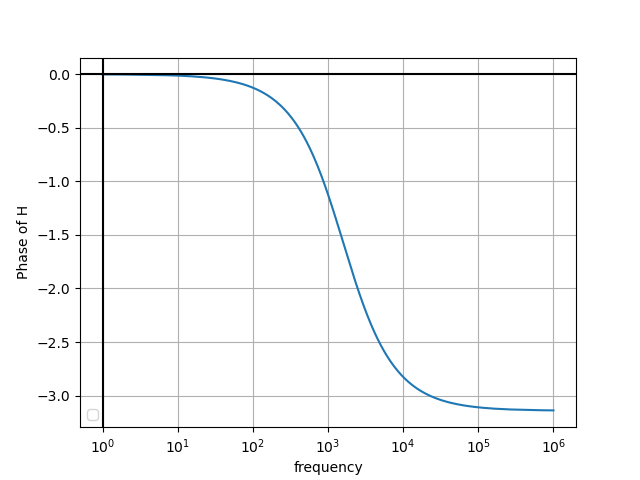
\includegraphics[width=\columnwidth]{2022/BM/38/figs/phase.png}
    \caption{Phase of H(f)}
    \label{Phase of H(f)}
\end{figure}
\begin{align}
    \angle {H(j\omega)} &= \tan^{-1}\brak{\frac{-\omega}{a}} - \tan^{-1}\brak{\frac{\omega}{a}}\\
    H(j\omega) &= \frac{e^{j\tan^{-1}\brak{\frac{-\omega}{a}}}}{e^{j\tan^{-1}\brak{\frac{\omega}{a}}}}\\
    &= \frac{\frac{a - j\omega}{\sqrt{a^2 + \omega^2}}}{\frac{a + j\omega}{\sqrt{a^2 + \omega^2}}}\\
    &= \frac{a - j\omega}{a + j\omega}
\end{align}
Substitute $s = j\omega$
\begin{align}
    u(t) &\system{\mathcal{L}} \frac{1}{s}\\
    Y(s) &= \frac{1}{s} \frac{a - s}{a + s}\\
    &= \frac{1}{s} - \frac{2}{a + s}\\
    \frac{1}{s} &\mathrel{\substack{\mathcal{L}^{-1}\\\longleftrightarrow}} u(t)\\
    \frac{1}{a + s} &\mathrel{\substack{\mathcal{L}^{-1}\\\longleftrightarrow}} e^{-at} u(t) \\
    y(t) &= (1-2e^{-at}) u(t)
\end{align}
Verification of laplace transform:
\begin{figure}[!h]
    \centering
    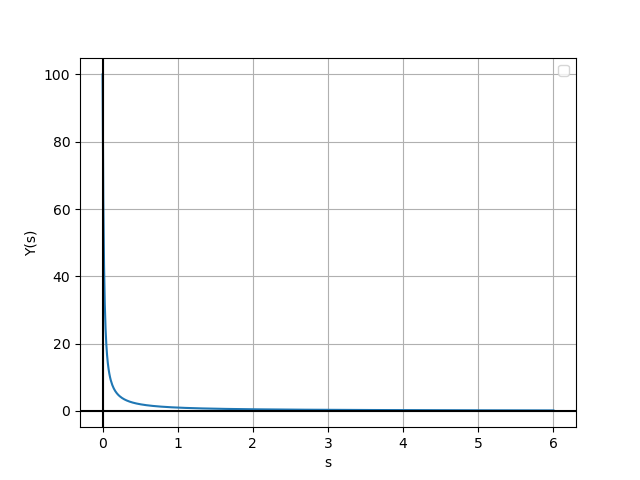
\includegraphics[width=\columnwidth]{2022/BM/38/figs/laplace_transform1.png}
    \caption{Laplace Transform of $u(t)$}
\end{figure}
\begin{figure}[!h]
    \centering
    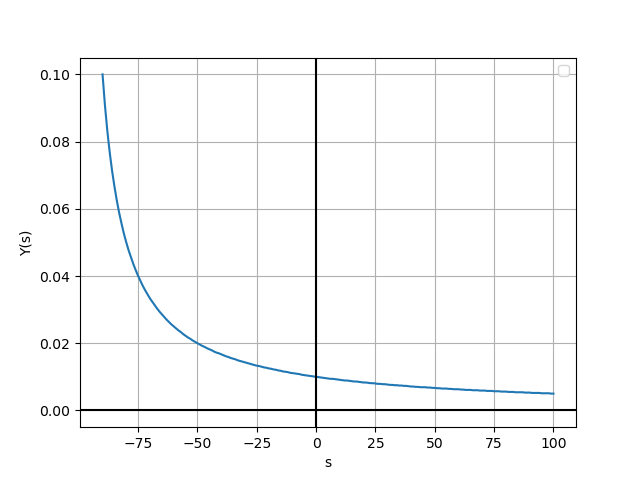
\includegraphics[width=\columnwidth]{2022/BM/38/figs/laplace_transform2.png}
    \caption{Laplace Transform $of e^{-at} u(t)$}
\end{figure}
\begin{align}
    \because y(t_d) &= 0 \\
    t_d &= 100 \ln{2} \micro s 
\end{align}
\begin{figure}[!h]
    \centering
    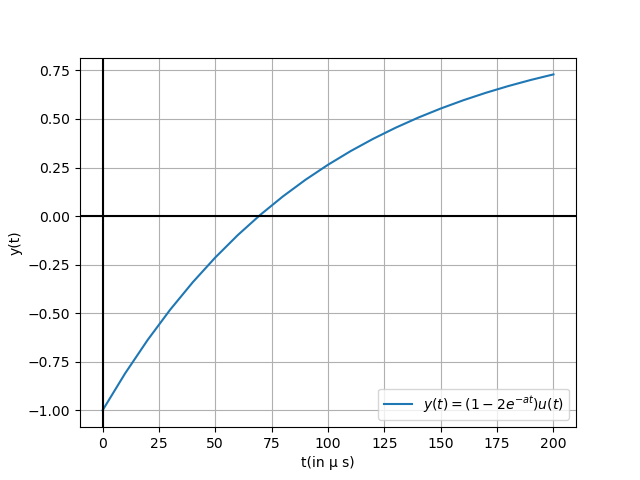
\includegraphics[width=\columnwidth]{2022/BM/38/figs/graph.png}
\end{figure}


\newpage

\item Consider the circuit shown in the figure with input V(t) in volts.The sinusoidal steady state current I(t) flowing through the circuit is shown graphically(where t is in seconds). The circuit element Z can be\rule{1.5cm}{0.15mm}.\hfill{GATE 2022 EC 39}
\begin{enumerate}
    \item a capacitor of 1 F
    \item an inductor of 1 H
    \item a capacitor of $\sqrt{3}$ H
    \item an inductor of $\sqrt{3}$ H
\end{enumerate}
\begin{circuitikz}
    \draw (0,0) node[ground]{};
    \draw (0,0) to [sV, l=$v(t)$] (0,3);
    \draw (0,3) to [resistor, l=$R$,i>^=$I(t)$] (3,3);
    \draw (3,3)to[european resistor,l=$Z$] (3,0);
    \draw (0,0)to (3,0);
  \end{circuitikz}
\begin{figure}[ht]
    \centering
    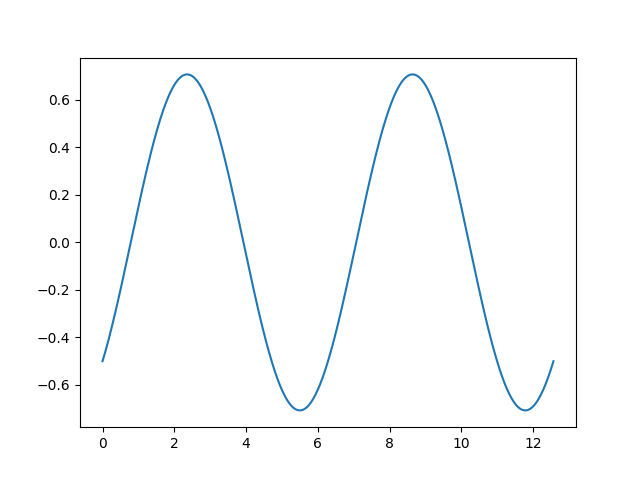
\includegraphics[width=\columnwidth]{2022/EC/39/figs/sin.png}
    \label{fig:GATE.2022.EC.39.1}
\end{figure}


\solution
\iffalse
\let\negmedspace\undefined
\let\negthickspace\undefined
\documentclass[journal,12pt,twocolumn]{IEEEtran}
\usepackage{cite}
\usepackage{amsmath,amssymb,amsfonts,amsthm}
\usepackage{algorithmic}
\usepackage{graphicx}
\usepackage{textcomp}
\usepackage{xcolor}
\usepackage{txfonts}
\usepackage{listings}
\usepackage{enumitem}
\usepackage{mathtools}
\usepackage{gensymb}
\usepackage{comment}
\usepackage[breaklinks=true]{hyperref}
\usepackage{tkz-euclide} 
\usepackage{listings}
\usepackage{gvv}                                        
\def\inputGnumericTable{}                                 
\usepackage[latin1]{inputenc}                                
\usepackage{color}                                            
\usepackage{array}                                            
\usepackage{longtable}                                       
\usepackage{calc}                                             
\usepackage{multirow}                                         
\usepackage{hhline}                                           
\usepackage{ifthen}                                           
\usepackage{lscape}
\usepackage{circuitikz}
\newtheorem{theorem}{Theorem}[section]
\newtheorem{problem}{Problem}
\newtheorem{proposition}{Proposition}[section]
\newtheorem{lemma}{Lemma}[section]
\newtheorem{corollary}[theorem]{Corollary}
\newtheorem{example}{Example}[section]
\newtheorem{definition}[problem]{Definition}
\newcommand{\BEQA}{\begin{eqnarray}}
\newcommand{\EEQA}{\end{eqnarray}}
\newcommand{\define}{\stackrel{\triangle}{=}}
\theoremstyle{remark}
\newtheorem{rem}{Remark}
\begin{document}
\parindent 0px

\bibliographystyle{IEEEtran}
\vspace{3cm}

\title{Assignment\\[1ex]GATE-EC-39}
\author{EE23BTECH11034 - Prabhat Kukunuri$^{}$% <-this % stops a space
}
\maketitle
\newpage
\bigskip

\renewcommand{\thefigure}{\theenumi}
\renewcommand{\thetable}{\theenumi}
\section{Question}
Consider the circuit shown in the figure with input V(t) in volts.The sinusoidal steady state current I(t) flowing through the circuit is shown graphically(where t is in seconds). The circuit element Z can be\rule{1.5cm}{0.15mm}.
\begin{enumerate}
    \item a capacitor of 1 F
    \item an inductor of 1 H
    \item a capacitor of $\sqrt{3}$ H
    \item an inductor of $\sqrt{3}$ H
\end{enumerate}
\begin{circuitikz}
    \draw (0,0) node[ground]{};
    \draw (0,0) to [sV, l=$v(t)$] (0,3);
    \draw (0,3) to [resistor, l=$R$,i>^=$I(t)$] (3,3);
    \draw (3,3)to[european resistor,l=$Z$] (3,0);
    \draw (0,0)to (3,0);
  \end{circuitikz}
\begin{figure}[ht]
    \centering
    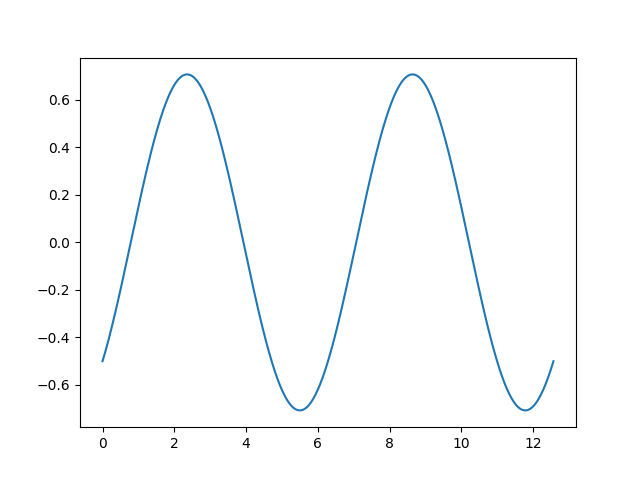
\includegraphics[width=\columnwidth]{2022/EC/39/figs/sin.png}
    \label{fig:GATE.2022.EC.39.1}
\end{figure}


\solution\\
\fi
\begin{table}[h]
    \centering
    \begin{tabular}{|p{2cm}|p{2.80cm}|p{2.70cm}|}
    \hline
    Symbol&Value&Description\\ \hline
    $$V\brak{t}$$&$$\sin{t}$$&Time varying voltage source\\\hline
    $$I\brak{t}$$&$$\sin{t-\frac{\pi}{4}}$$&Current flowing in the circuit\\\hline
    $$R$$&$$1\ohm$$&Resistor in series to Z\\\hline
    $$Z$$&$$Z$$&Circuit element\\\hline
    \end{tabular}
    \caption{Variable description}
    \label{tab:GATE.2022.EC.39.1}
\end{table}\\
The current through the circuit can be expressed as
\begin{align}
    I(t)=\sin\brak{t-\frac{\pi}{4}}
\end{align}
Since, the voltage seems to be leading the current the circuit element z is an inductor with inductance L.\\
Applying KVL in the circuit,
\begin{align}
    R.I\brak{t}+L\frac{dI\brak{t}}{dt}=sin\brak{t}
\end{align}
Applying Fourier transform to the differential equation,
\begin{align}
    &R.I\brak{s}+sL.I\brak{s}-\frac{1}{s^2+1}=0\\
    &I\brak{s}\brak{R+sL}=\frac{1}{s^2+1}\\
    &\sin\brak{at+b}\system{L}\frac{a\cos\brak{b}+s\sin\brak{b}}{a^{2}+s^{2}}\\
    &\sin\brak{t-\frac{\pi}{4}}\system{L}\frac{1-s}{2\brak{s^2+1}}\\
    &\frac{1-s}{2\brak{s^2+1}}\brak{R+sL}=\frac{1}{s^2+1}
\end{align}
Upon plugging in R=1$\ohm$,
\begin{align}
   L=\frac{1}{s}
\end{align}
Applying inverse Laplace,
\begin{align}
    L=1H
\end{align}

Appendix\\
Laplace transform of $\sin\brak{at+b}$ is as follows,
\begin{align}
    &\sin\brak{at+b}\system{L}\int_{0}^{\infty}\sin\brak{at+b}e^{-st}dt\\
    &\int_{0}^{\infty}\sin\brak{at+b}e^{-st}dt=\cos{b}\int_{0}^{\infty}\sin\brak{at}e^{-st}dt+\sin{b}\int_{0}^{\infty}\cos\brak{at}e^{-st}dt\\
    &\int_{0}^{\infty}\cos\brak{at}e^{-st}dt=\frac{e^{-st}}{a}sin{at}\Bigg|_{0}^{\infty}+\frac{s}{a}\int_{0}^{\infty}\sin\brak{at}e^{-st}dt\\
    &\int_{0}^{\infty}\cos\brak{at}e^{-st}dt=\frac{s}{a}\int_{0}^{\infty}\sin\brak{at}e^{-st}dt\label{eq:GATE.2022.EC.39.2}\\
    &\int_{0}^{\infty}\cos\brak{at}e^{-st}dt=\frac{s}{a}\brak{\frac{-e^{-st}}{a}cos{at}\Bigg|_{0}^{\infty}+\frac{s}{a}\int_{0}^{\infty}\cos\brak{at}e^{-st}dt}\\
    &\int_{0}^{\infty}\cos\brak{at}e^{-st}dt=\frac{s}{a^2}+\frac{s^2}{a^2}\int_{0}^{\infty}\cos\brak{at}e^{-st}dt
\end{align}
\begin{align}
    &\int_{0}^{\infty}\cos\brak{at}e^{-st}dt=\frac{s}{s^2+a^2},s>0
\end{align}
From \eqref{eq:GATE.2022.EC.39.2} we can say,
\begin{align}
    &\int_{0}^{\infty}\sin\brak{at}e^{-st}dt=\frac{a}{s^2+a^2},s>0\\
    &\therefore \sin\brak{at+b}\system{L}\frac{s\sin{b}+a\cos{b}}{s^2+a^2}
\end{align}
%\end{document}

\pagebreak
\newpage

\item Consider the differential equation
    $\frac{dy}{dx} = 4(x+2) - y$ 
For the initial condition $y = 3$ at $x = 1$, the value of $y$ at $x = 1.4$ obtained using Euler's method with a step-size of 0.2 is ? (\textit{round off to one decimal place})
\hfill{(GATE CE 2022)}\\
\solution
\iffalse
\let\negmedspace\undefined
\let\negthickspace\undefined
\documentclass[journal,12pt,onecolumn]{IEEEtran}
\usepackage{cite}
\usepackage{amsmath,amssymb,amsfonts,amsthm}
\usepackage{algorithmic}
\usepackage{graphicx}
\usepackage{textcomp}
\usepackage{xcolor}
\usepackage{txfonts}
\usepackage{listings}
\usepackage{enumitem}
\usepackage{circuitikz}
\usepackage{mathtools}
\usepackage{gensymb}
\usepackage{comment}
\usepackage[breaklinks=true]{hyperref}
\usepackage{tkz-euclide} 
\usepackage{listings}
\usepackage{gvv}    
\usepackage{enumitem}
\usepackage{amsmath}
\def\inputGnumericTable{}                                 
\usepackage[latin1]{inputenc}                                
\usepackage{color}                                            
\usepackage{array}                                            
\usepackage{longtable}                                       
\usepackage{calc}                                             
\usepackage{multirow}                                         
\usepackage{hhline}                                           
\usepackage{ifthen}                                           
\usepackage{lscape}
\usepackage{tabularx}
\usepackage[italicdiff]{physics}
\usepackage{mathrsfs}


\newtheorem{theorem}{Theorem}[section]
\newtheorem{problem}{Problem}
\newtheorem{proposition}{Proposition}[section]
\newtheorem{lemma}{Lemma}[section]
\newtheorem{corollary}[theorem]{Corollary}
\newtheorem{example}{Example}[section]
\newtheorem{definition}[problem]{Definition}
\newcommand{\BEQA}{\begin{eqnarray}}
\newcommand{\EEQA}{\end{eqnarray}}
\newcommand{\define}{\stackrel{\triangle}{=}}
\theoremstyle{remark}
\newtheorem{rem}{Remark}
\begin{document}
\bibliographystyle{IEEEtran}
\vspace{3cm}

\title{GATE:2022 - CE 48 }
\author{EE23BTECH11025 - Anantha Krishnan $^{}$% <-this % stops a space
}
\maketitle
\bigskip



\section{question}

Consider the differential equation
\begin{align}
    \frac{dy}{dx} = 4(x+2) - y \notag
\end{align}
For the initial condition $y = 3$ at $x = 1$, the value of $y$ at $x = 1.4$ obtained using Euler's method with a step-size of 0.2 is ? (\textit{round off to one decimal place})
\hfill{(GATE CE 2022)}\\
 



\textbf{Solutions :}
\fi
\begin{table}[ht!]
\centering
\begin{tabular}{ |c|c|c| } 
 \hline
Symbols & Description & Values  \\
\hline
$R$ & Residue Formula &$\frac{1}{\brak {m-1}!}\lim\limits_{s\to a}\frac{d^{m-1}}{ds^{m-1}}\brak {{(s-a)}^{m}f\brak se^{st}}$\\
 \hline
 $\phi(x)$ & Transformation of $y(x)$ & $y(x+1)$\\
 \hline
$g(x)$ & Euler's Approximated function of f(x) & $g_{(n-1)}(x) + hf'\brak{x_{n-1},y_{n-1}}$\\
 \hline
 $h$ & Step-size & $0.2$\\
 \hline
\end{tabular}
\caption{Parameters, Descriptions, and Values}
\label{table:ee25-ce48-gate2022}
\end{table}





\begin{enumerate}
    \item Solution of the differential:\\
 Applying the transformation from table \ref{table:ee25-ce48-gate2022} and laplace transform 
    \begin{align}
             s\mathscr{L}\brak{\phi(x)} - \phi(0) &= 4\brak{\frac{1}{s^2}+\frac{3}{s}}-\mathscr{L}\brak{\phi(x)}\\
             \mathscr{L}\brak{\phi(x)} &= \frac{3}{s+1} + 4\brak{\frac{1}{s^2\brak{s+1}}+\frac{3}{s\brak{s+1}}}\\
             &=\frac{-5}{s+1} + \frac{8}{s} + \frac{4}{s^2}
    \end{align}
\item  Inverse Laplace Transform:\\
Using Bromwich integrals and extension of Jordans lemma :
\begin{align}
    \phi(t) &= \frac{1}{2\pi j}\int_{c-j\infty}^{c+j\infty}\mathscr{L}\brak{\phi(x)}e^{st}\,dt , c > 0\\
     &= \frac{1}{2\pi j}\int_{c-j\infty}^{c+j\infty}\brak{\frac{-5}{s+1} + \frac{8}{s} + \frac{4}{s^2}}e^{st}\,dt
\end{align}
Here, the poles $s=-1$ (non repeated, $m=1$) and $s=0$ (repeated, $m=2$) lie inside a semicircle for some $c>0$. Using method of residues from \ref{table:ee25-ce48-gate2022}:
\begin{align}
    R_1 &= \lim\limits_{s\to -1}\brak {{\brak{s+1}}\brak{\frac{-5}{s+1}}e^{st}} \\
    &= -5e^{-t}\\
   R_2 &= \lim\limits_{s\to 0}\brak {{\brak{s}}\brak{\frac{8}{s}}e^{st}}\\
   &= 8\\
 R_3&=\frac{1}{\brak {1}!}\lim\limits_{s\to 0}\frac{d}{dz}\brak {{(s)}^{2}\brak{\frac{4}{s^2}}e^{st}}\\
 &=4t\\
\phi(t) &= R_1 + R_2 + R_3\\
&= -5e^{-t} + 8 + 4t
\end{align}
Reverting to $y(x)$ , we get :
\begin{align}
    y(x) &= -5e^{-x+1} + x + 4x
\end{align}
\end{enumerate}
Now, approaching to $y(1.4)$ using euler's approximation from \ref{table:ee25-ce48-gate2022}
\begin{align}
    g_{\brak{1.2}} &= 3 + \brak{0.2}f'\brak{1,3}\\
    &=4.8\\
    g_{\brak{1.4}} &= 4.8 +\brak{0.2}f'\brak{1.2,4.8}\\
    &= 6.4\\
    &\implies y(1.4) \approx 6.4 
\end{align}





    \begin{figure}[!ht]    
    \centering
\graphicspath{ {2022/CE/48/figs/} }
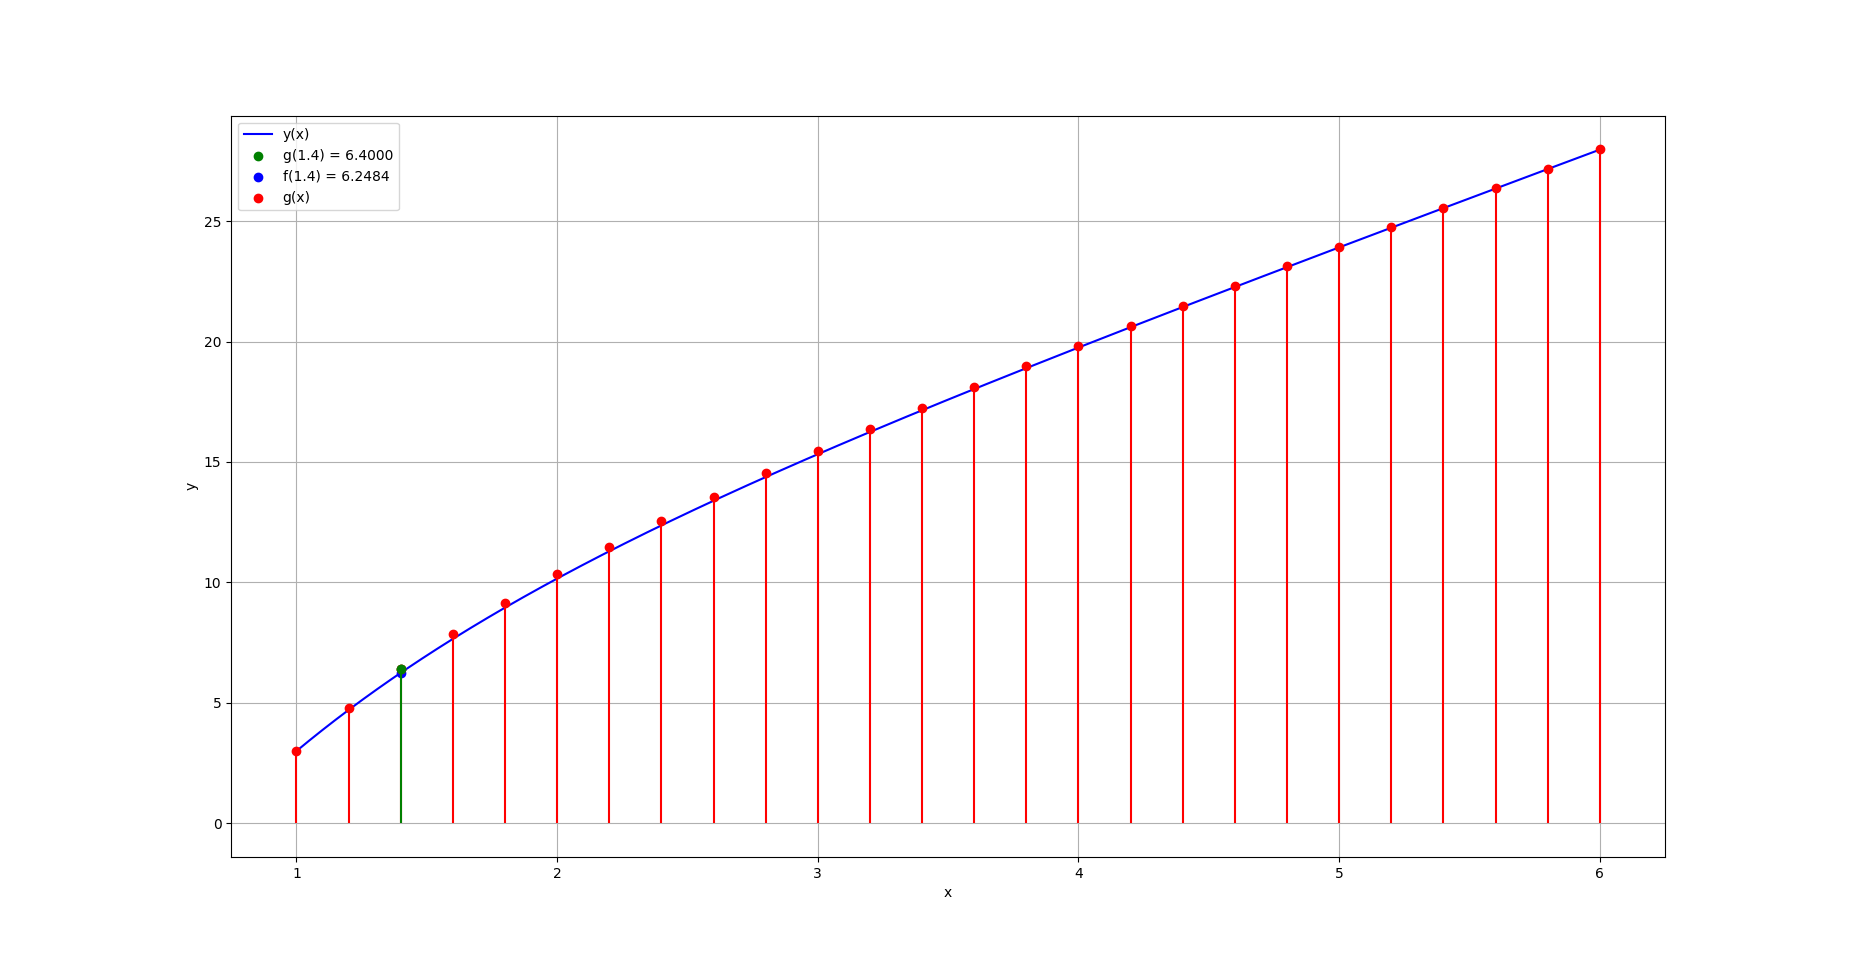
\includegraphics[width=\columnwidth]{graph_1}
\caption{ Euler's approximated function vs Original function  }
\label{graph:ee25-gate3-graph}
\end{figure}



\pagebreak

\item A unity-gain negative-feedback control system has a loop-gain $L\brak{s}$ given by
\begin{align}
    L\brak{s} = \frac{6}{s\brak{s-5}}
\end{align}
The closed loop system is \rule{1cm}{0.15mm}
\begin{enumerate}
    \item Causal and stable
    \item Causal and unstable
    \item Non-causal and stable
    \item Non-causal and unstable
\end{enumerate}
\hfill(GATE IN 2022)\\
\solution
\iffalse
\let\negmedspace\undefined
\let\negthickspace\undefined
\documentclass[journal,12pt,twocolumn]{IEEEtran}
\usepackage{cite}
\usepackage{amsmath,amssymb,amsfonts,amsthm}
\usepackage{algorithmic}
\usepackage{graphicx}
\usepackage{textcomp}
\usepackage{xcolor}
\usepackage{txfonts}
\usepackage{listings}
\usepackage{enumitem}
\usepackage{mathtools}
\usepackage{gensymb}
\usepackage{comment}
\usepackage[breaklinks=true]{hyperref}
\usepackage{tkz-euclide} 
\usepackage{listings}
\usepackage{gvv}                                        
\def\inputGnumericTable{}                                 
\usepackage[latin1]{inputenc}                                
\usepackage{color}                                            
\usepackage{array}                                            
\usepackage{longtable}                                       
\usepackage{calc}                                             
\usepackage{multirow}                                         
\usepackage{hhline}                                           
\usepackage{ifthen}                                           
\usepackage{lscape}
\usepackage{placeins}
\usepackage{xparse}


\newtheorem{theorem}{Theorem}[section]
\newtheorem{problem}{Problem}
\newtheorem{proposition}{Proposition}[section]
\newtheorem{lemma}{Lemma}[section]
\newtheorem{corollary}[theorem]{Corollary}
\newtheorem{example}{Example}[section]
\newtheorem{definition}[problem]{Definition}
\newcommand{\BEQA}{\begin{eqnarray}}
\newcommand{\EEQA}{\end{eqnarray}}
\newcommand{\define}{\stackrel{\triangle}{=}}
\theoremstyle{remark}
\newtheorem{rem}{Remark}

\graphicspath{ {./figs/} } 

\begin{document}

\bibliographystyle{IEEEtran}
\vspace{3cm}

\Large\title{GATE 2022 IN 15}
\large\author{EE23BTECH11032 - Kaustubh Parag Khachane $^{*}$% <-this % stops a space
}
\maketitle
\newpage
\bigskip

\renewcommand{\thefigure}{\theenumi}
\renewcommand{\thetable}{\theenumi}
\large\textbf{Question GATE 22 IN 15} :\\
A unity-gain negative-feedback control system has a loop-gain $L\brak{s}$ given by
\begin{align}
    L\brak{s} = \frac{6}{s\brak{s-5}}
\end{align}
The closed loop system is \rule{1cm}{0.15mm}
\begin{enumerate}
    \item Causal and stable
    \item Causal and unstable
    \item Non-causal and stable
    \item Non-causal and unstable
\end{enumerate}
\hfill(GATE IN 2022)\\
\solution\\
\fi
\begin{table}[!ht] 
\centering
\setlength{\extrarowheight}{8pt}
\begin{tabular}{|l|l|l|}
    \hline
    \textbf{Parameter} & \textbf{Description} & \textbf{Value} \\
    \hline
     $L\brak{s}$ & Forward loop transfer function & $\frac{6}{s\brak{s-5}}$ \\\hline
     $H\brak{s}$ & Feedback path transferfunction & 1 \\\hline
     $T\brak{s}$ & Transfer function & $\frac{L\brak{s}}{1 + L\brak{s}H\brak{s}}$ \\\hline
    \end{tabular}
  \vspace{4mm}
 \caption{Parameter Table}
 \label{tab:table0_in15}
\end{table}

From \tabref{tab:table0_in15}, the transfer function of the system is given by,
\begin{align}
    T\brak{s} &= \frac{\frac{6}{s\brak{s-5}}}{1 + 1\frac{6}{s\brak{s-5}}}\\
    &= \frac{6}{s^2 - 5s + 6}
\end{align}
The poles of the system are given by the roots of the denominator of transfer function,
\begin{align}
    s^2 - 5s + 6 = 0
\end{align}
$\therefore$ The poles of the system are $s = 2$ and $s = 3$.\\
As the poles are positive, the output will increase without bound, causing the system to be unstable.
\\The transfer function of the system is ,
\begin{align}
    T\brak{s} = \frac{6}{\brak{s-2}\brak{s-3}}
\end{align}
Clearly, it is dependent only on the past values. Hence, the system is causal.
\\Thus the correct option is B. The system is causal and unstable.
\begin{figure}[!ht]
\centering
\begin{center}
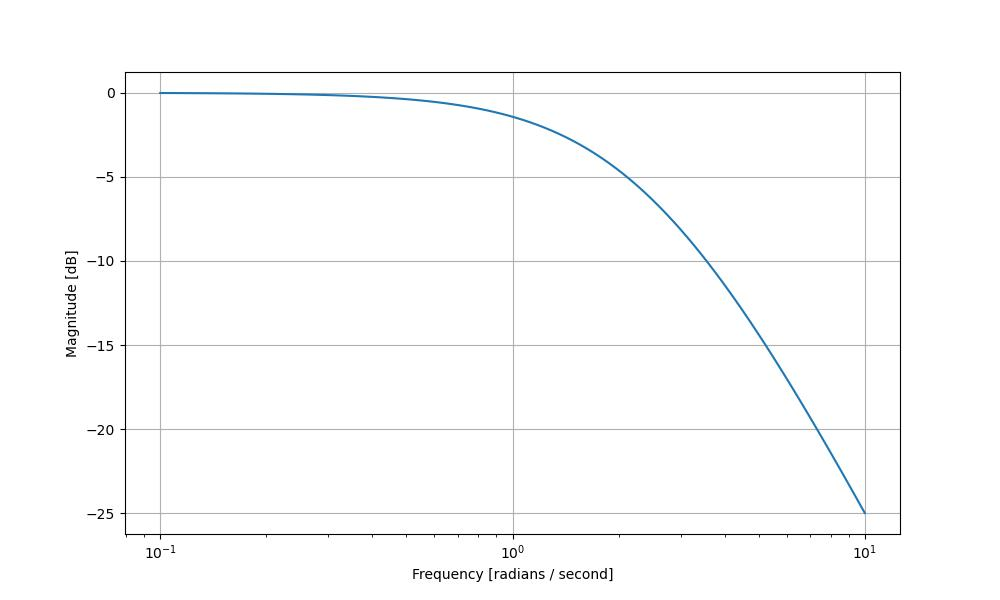
\includegraphics[width=\columnwidth]{2022/IN/15/figs/Figure_1.jpg}
\end{center}
\caption{Magnitude plot for the transfer function}
\end{figure}
\begin{figure}[!ht]
\centering
\begin{center}
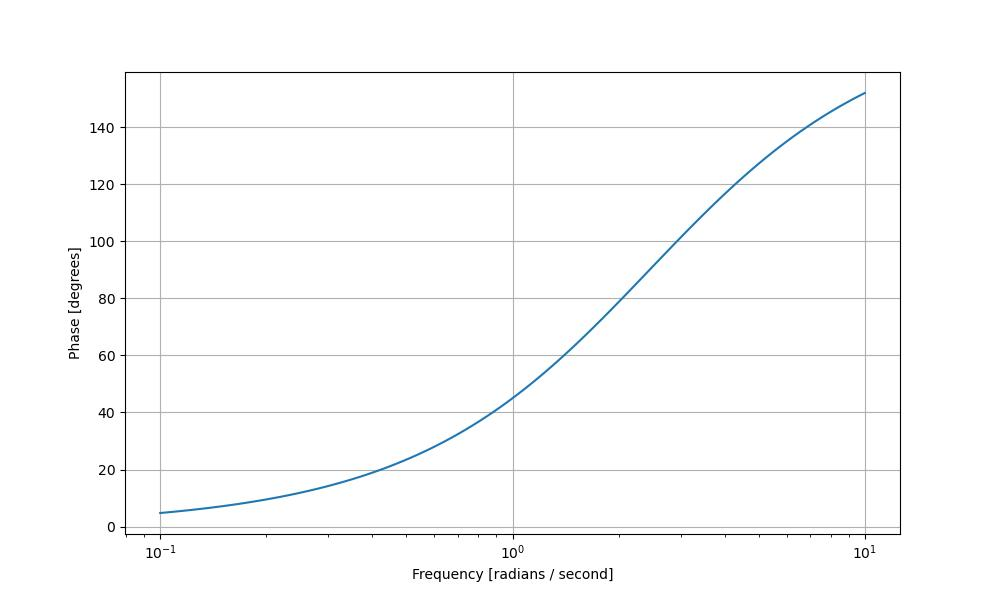
\includegraphics[width=\columnwidth]{2022/IN/15/figs/Figure_2.jpg}
\end{center}
\caption{Phase plot for the transfer function}
\end{figure}

\newpage

\item
If 
\begin{align}
 g(t) &= \frac{df(t)}{dt} \\
 F(s) &= \frac{1+s}{s^2+12s+32} 
\end{align} 
where $F(s)$ is the Laplace transform of the function $f(t)$, then what is the value of $g(t)$ at $t=0$ ?\\
\hfill(GATE BM 2022)\\
\solution
\iffalse
\documentclass[journal,12pt,twocolumn]{IEEEtran}
\usepackage{cite}
\usepackage{amsmath,amssymb,amsfonts,amsthm}
\usepackage{algorithmic}
\usepackage{graphicx}
\usepackage{textcomp}
\usepackage{xcolor}
\usepackage{txfonts}
\usepackage{listings}
\usepackage{enumitem}
\usepackage{mathtools}
\usepackage{gensymb}
\usepackage{comment}
\usepackage[breaklinks=true]{hyperref}
\usepackage{tkz-euclide}
\usepackage{braket}
\def\inputGnumericTable{}
\usepackage[latin1]{inputenc}
\usepackage{color}
\usepackage{array}
\usepackage{longtable}
\usepackage{calc}
\usepackage{multirow}
\usepackage{hhline}
\usepackage{ifthen}
\usepackage{lscape}
\usepackage{gvv} 

\newtheorem{theorem}{Theorem}[section]
\newtheorem{problem}{Problem}
\newtheorem{proposition}{Proposition}[section]
\newtheorem{lemma}{Lemma}[section]
\newtheorem{corollary}[theorem]{Corollary}
\newtheorem{example}{Example}[section]
\newtheorem{definition}[problem]{Definition}
\newcommand{\BEQA}{\begin{eqnarray}}
\newcommand{\EEQA}{\end{eqnarray}}
\newcommand{\define}{\stackrel{\triangle}{=}}
\theoremstyle{remark}
\newtheorem{rem}{Remark}

\begin{document}

\bibliographystyle{IEEEtran}
\vspace{3cm}

\title{GATE 2022 BM-42}
\author{EE23BTECH11201 - Abburi Tanusha$^{*}$% <-this % stops a space
}
\maketitle
\newpage
\bigskip

\renewcommand{\thefigure}{\theenumi}
\renewcommand{\thetable}{\theenumi}

\vspace{3cm}

\maketitle
\textbf{Question:} 
If 
\begin{align}
 g(t) &= \frac{df(t)}{dt} \\
 F(s) &= \frac{1+s}{s^2+12s+32} 
\end{align} 
where $F(s)$ is the Laplace transform of the function $f(t)$, then what is the value of $g(t)$ at $t=0$ ?\\
\hfill(GATE BM 2022)\\
\textbf{Solution:} 
\fi
\begin{table}[h!]
\centering
\resizebox{6cm}{!}{

\begin{tabular}{|c|c|c|}
\hline
\textbf{Value} & \textbf{Parameter} & \textbf{Description} \\
\hline
$g(t)$ & $\frac{df(t)}{dt}$ & Derivative of $f(t)$ with respect to $t$ \\
\hline
$F(s)$ & $\frac{1+s}{s^2+12s+32}$ & Laplace transform of the function $f(t)$ \\
\hline

\end{tabular}



}
\caption{Given Parameters}
\label{tab:tanu_tabel}
\end{table}

Using Initial value Theorem 
\begin{align}
    f(0) &= \lim_{s \to \infty} sF(s) \\
         &= \lim_{s \to \infty} \frac{s(s+1)}{s^2 + 12s + 32} \\
         &= 1 \\
    G(s) &= sF(s) - f(0) \\
         &= \frac{s(s+1)}{s^2 + 12s + 32} - 1 \\
         &= \frac{s^2 + s - (s^2 + 12s + 32)}{s^2 + 12s + 32} \\
         G(s) &= \frac{-11s - 32}{s^2 + 12s + 32} 
\end{align}
Using Partial fraction decomposition 
\begin{align}
      G(s)   &= \frac{A}{s+4} + \frac{B}{s+8}  \\
    -11s - 32 &= A(s+8) + B(s+4) \\
    -11s - 32 &= (A + B)s + (8A + 4B)
\end{align}
Equating coefficients:
\begin{align}
     -11 &= A + B \\
    -32 &= 8A + 4B
\end{align}
By solving these equations , we get 
\begin{align}
    A &= 3 \\
    B &= -14 \\
    G(s) &=\frac{3}{s+4} - \frac{14}{s+8} ; \quad Re(s) > -4
\end{align}
Inverse Laplace transform of $G(s)$ 
\begin{align}
g(t) &=\mathcal{L}^{-1}\brak{\frac{3}{s+4}} -\mathcal{L}^{-1}\brak{\frac{14}{s+8}} \\
   &= 3e^{-4t} - 14e^{-8t} \\
g(0) &= 3e^{-4 \cdot 0} - 14e^{-8 \cdot 0} \\
         &= 3 - 14 \\
         &= -11
\end{align}
Verifying g(0) by Initial value theorem
\begin{align}
    g(0) &= \lim_{s \to \infty} sG(s) \\
         &= \lim_{s \to \infty} s \cdot \frac{-11s - 32}{s^2 + 12s + 32} \\
         &= \lim_{s \to \infty} \frac{-11 - \frac{32}{s}}{1 + \frac{12}{s} + \frac{32}{s^2}} \\
         &= \lim_{s \to \infty} \frac{-11}{1} \\
         &= -11
\end{align}
The value of $g(t)$ at $t=0$ is $-11$.
\begin{figure}[h!]
\centering
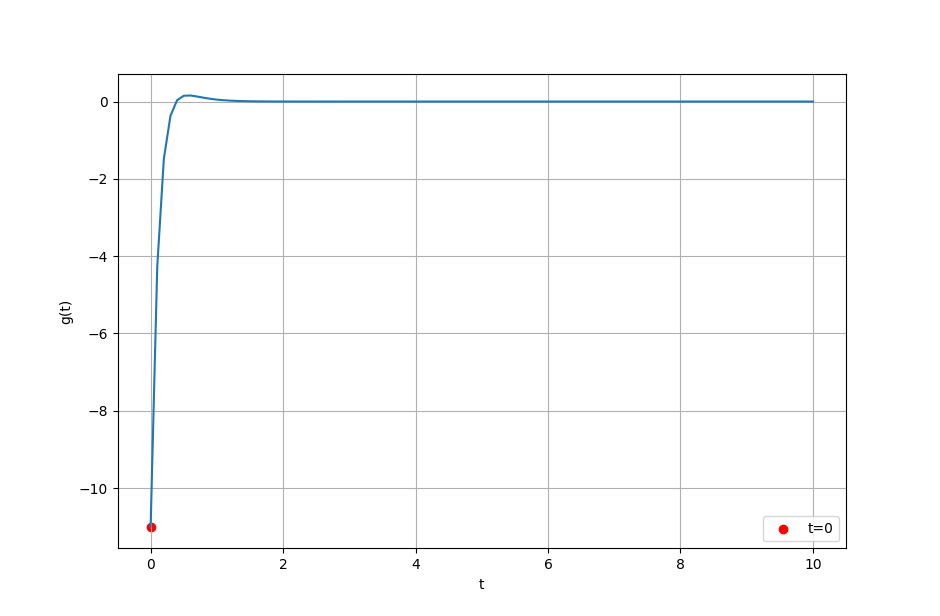
\includegraphics[width=\columnwidth]{2022/BM/42/figs/stem_plot.png}
\caption{Plot $g(t)$ vs $t$ }
\label{fig:tansh_plott}
\end{figure}
%\end{document}


\pagebreak

\item Let $y(x)$ be the solution of the differential equation 
\begin{align}
y^{''} - 4y^{'} -12y &= 3e^{5x} 
 \label{eq:ishitha.g22.nm.50.1.eq}
\end{align}
satisfying $y(0)=\frac{18}{7}$ and $y^{'}(0)=\frac{-1}{7}$. \\
Then $y(1)$ is \underline{\hspace{2.5cm}}  (rounded off to nearest integer).      \hfill{GATE NM 2022 }\\
\solution
\iffalse
\let\negmedspace\undefined
\let\negthickspace\undefined
\documentclass[journal,12pt,twocolumn]{IEEEtran}
\usepackage{cite}
\usepackage{amsmath,amssymb,amsfonts,amsthm}
\usepackage{algorithmic}
\usepackage{graphicx}
\usepackage{textcomp}
\usepackage{xcolor}
\usepackage{txfonts}
\usepackage{listings}
\usepackage{enumitem}
\usepackage{mathtools}
\usepackage{gensymb}
\usepackage[breaklinks=true]{hyperref}
\usepackage{tkz-euclide} % loads  TikZ and tkz-base
\usepackage{listings}



\newtheorem{theorem}{Theorem}[section]
\newtheorem{problem}{Problem}
\newtheorem{proposition}{Proposition}[section]
\newtheorem{lemma}{Lemma}[section]
\newtheorem{corollary}[theorem]{Corollary}
\newtheorem{example}{Example}[section]
\newtheorem{definition}[problem]{Definition}
%\newtheorem{thm}{Theorem}[section] 
%\newtheorem{defn}[thm]{Definition}
%\newtheorem{algorithm}{Algorithm}[section]
%\newtheorem{cor}{Corollary}
\newcommand{\BEQA}{\begin{eqnarray}}
\newcommand{\EEQA}{\end{eqnarray}}
\newcommand{\define}{\stackrel{\triangle}{=}}
\theoremstyle{remark}
\newtheorem{rem}{Remark}
%\bibliographystyle{ieeetr}
\begin{document}
%
\providecommand{\pr}[1]{\ensuremath{\Pr\left(#1\right)}}
\providecommand{\prt}[2]{\ensuremath{p_{#1}^{\left(#2\right)} }}        % own macro for this question
\providecommand{\qfunc}[1]{\ensuremath{Q\left(#1\right)}}
\providecommand{\sbrak}[1]{\ensuremath{{}\left[#1\right]}}
\providecommand{\lsbrak}[1]{\ensuremath{{}\left[#1\right.}}
\providecommand{\rsbrak}[1]{\ensuremath{{}\left.#1\right]}}
\providecommand{\brak}[1]{\ensuremath{\left(#1\right)}}
\providecommand{\lbrak}[1]{\ensuremath{\left(#1\right.}}
\providecommand{\rbrak}[1]{\ensuremath{\left.#1\right)}}
\providecommand{\cbrak}[1]{\ensuremath{\left\{#1\right\}}}
\providecommand{\lcbrak}[1]{\ensuremath{\left\{#1\right.}}
\providecommand{\rcbrak}[1]{\ensuremath{\left.#1\right\}}}
\newcommand{\sgn}{\mathop{\mathrm{sgn}}}
\providecommand{\abs}[1]{\left\vert#1\right\vert}
\providecommand{\res}[1]{\Res\displaylimits_{#1}} 
\providecommand{\norm}[1]{\left\lVert#1\right\rVert}
%\providecommand{\norm}[1]{\lVert#1\rVert}
\providecommand{\mtx}[1]{\mathbf{#1}}
\providecommand{\mean}[1]{E\left[ #1 \right]}
\providecommand{\cond}[2]{#1\middle|#2}
\providecommand{\fourier}{\overset{\mathcal{F}}{ \rightleftharpoons}}
\newenvironment{amatrix}[1]{%
  \left(\begin{array}{@{}*{#1}{c}|c@{}}
}{%
  \end{array}\right)
}
%\providecommand{\hilbert}{\overset{\mathcal{H}}{ \rightleftharpoons}}
%\providecommand{\system}{\overset{\mathcal{H}}{ \longleftrightarrow}}
	%\newcommand{\solution}[2]{\textbf{Solution:}{#1}}
\newcommand{\solution}{\noindent \textbf{Solution: }}
\newcommand{\cosec}{\,\text{cosec}\,}
\providecommand{\dec}[2]{\ensuremath{\overset{#1}{\underset{#2}{\gtrless}}}}
\newcommand{\myvec}[1]{\ensuremath{\begin{pmatrix}#1\end{pmatrix}}}
\newcommand{\mydet}[1]{\ensuremath{\begin{vmatrix}#1\end{vmatrix}}}
\newcommand{\myaugvec}[2]{\ensuremath{\begin{amatrix}{#1}#2\end{amatrix}}}
\providecommand{\rank}{\text{rank}}
\providecommand{\pr}[1]{\ensuremath{\Pr\left(#1\right)}}
\providecommand{\qfunc}[1]{\ensuremath{Q\left(#1\right)}}
	\newcommand*{\permcomb}[4][0mu]{{{}^{#3}\mkern#1#2_{#4}}}
\newcommand*{\perm}[1][-3mu]{\permcomb[#1]{P}}
\newcommand*{\comb}[1][-1mu]{\permcomb[#1]{C}}
\providecommand{\qfunc}[1]{\ensuremath{Q\left(#1\right)}}
\providecommand{\gauss}[2]{\mathcal{N}\ensuremath{\left(#1,#2\right)}}
\providecommand{\diff}[2]{\ensuremath{\frac{d{#1}}{d{#2}}}}
\providecommand{\myceil}[1]{\left \lceil #1 \right \rceil }
\newcommand\figref{Fig.~\ref}
\newcommand{\systemL}[1]{\stackrel{#1}{\xleftrightarrow{\mathcal{L}}}}
\newcommand{\systemLinv}[1]{\stackrel{#1}{\xleftrightarrow{\mathcal{L}^{-1}}}}


\newcommand\tabref{Table~\ref}
\newcommand{\sinc}{\,\text{sinc}\,}
\newcommand{\rect}{\,\text{rect}\,}
%%
%	%\newcommand{\solution}[2]{\textbf{Solution:}{#1}}
%\newcommand{\solution}{\noindent \textbf{Solution: }}
%\newcommand{\cosec}{\,\text{cosec}\,}
%\numberwithin{equation}{section}
%\numberwithin{equation}{subsection}
%\numberwithin{problem}{section}
%\numberwithin{definition}{section}
%\makeatletter
%\@addtoreset{figure}{problem}
%\makeatother

%\let\StandardTheFigure\thefigure
\let\vec\mathbf


\bibliographystyle{IEEEtran}
\title{ GATE NM-50 2022}
\author{EE23BTECH11011- Batchu Ishitha$^{*}$% <-this % stops a space
}
\maketitle




\bigskip

\renewcommand{\thefigure}{\theenumi}
\renewcommand{\thetable}{\theenumi}
%\renewcommand{\theequation}{\theenumi}

Q:  Let $y(x)$ be the solution of the differential equation 
\begin{align}
y^{''} - 4y^{'} -12y &= 3e^{5x} 
 \label{eq:ishitha.g22.nm.50.1.eq}
\end{align}
satisfying $y(0)=\frac{18}{7}$ and $y^{'}(0)=\frac{-1}{7}$. \\
Then $y(1)$ is \underline{\hspace{2.5cm}}  (rounded off to nearest integer).      \hfill{GATE NM 2022 }

\solution
\fi
\begin{table}[!ht]    
    \centering
    \resizebox{9cm}{1cm}{
        \begin{tabular}[12pt]{ |c| c|c|}
    \hline
    \textbf{Parameter} & \textbf{Description} & \textbf{Value}\\ 
    \hline
    $y^{''} -  4y^{'} -12y = 3e^{5x}$ & Differential equation & none\\
    \hline
    $y\brak{x}$ &Solution of  differential equation & $y(0)=\frac{18}{7}$\\
    \hline
    $y^{'}\brak{x}$ & First order derivative of solution of differential equation & $y^{'}\brak{0}=\frac{-1}{7}$\\
    \hline
     \end{tabular} 
 
    }
    \caption{Input Parameters}
    \label{table:ishitha.g22.nm.50.t1}
\end{table}

\begin{equation}
y^{''}(t) \systemL{} s^{2}Y(s)-sy(0)-y^{'}(0) \\ \label{eq:ishitha.g22.nm.50.2.eq}
\end{equation}

\begin{equation}
y^{'}(t)  \systemL{} sY(s)-y(0) \\ \label{eq:ishitha.g22.nm.50.3.eq}
\end{equation}

\begin{equation}
y(t)     \systemL{}   Y(s) \\ \label{eq:ishitha.g22.nm.50.4.eq}
\end{equation}

\begin{equation}
e^{at}   \systemL{}  \frac{1}{s-a} \\ \label{eq:ishitha.g22.nm.50.5.eq}
\end{equation}

Applying Laplace transform on both sides of  ~\eqref{eq:ishitha.g22.nm.50.1.eq},
\begin{align}
\mathcal{L}\brak{y^{''}(t) - 4y^{'}(t) -12y(t)}&=\mathcal{L}\brak{3e^{5x}}
\end{align}

From ~\eqref{eq:ishitha.g22.nm.50.2.eq},~\eqref{eq:ishitha.g22.nm.50.3.eq},~\eqref{eq:ishitha.g22.nm.50.4.eq},~\eqref{eq:ishitha.g22.nm.50.5.eq}
\begin{align}
Y(s)\brak{s^{2}-4s-12} -y(0)\brak{s-4} -y^{'}(0) &= \frac{3}{s-5} \\
Y(s)\brak{s^{2}-4s-12} - \frac{\brak{18s -73 }}{7}  &=\frac{3}{(s-5)} \\
Y(s) &= \frac{3}{(s-5)\brak{s^{2}-4s-12}} + \frac{\brak{18s -73 }}{7\brak{s^{2}-4s-12} } 
\implies Y(s) = \frac{1}{\brak{s-6}} -\frac{3}{7\brak{s-5}} + \frac{1}{\brak{s+2}} 
\label{eq:ishitha.g22.nm.50.6.eq}
\end{align}


\begin{equation}
\frac{1}{s-a}   \systemLinv{}  e^{at}  \\ \label{eq:ishitha.g22.nm.50.7.eq}
\end{equation}
Now finding Inverse Laplace Transform on both sides of ~\eqref{eq:ishitha.g22.nm.50.6.eq} ,

From ~\eqref{eq:ishitha.g22.nm.50.7.eq}
\begin{align}
\implies y(t) &= \brak{e^{6t} -\frac{3}{7}e^{5t} + 2e^{-2t}}u(t)
\implies y(1) &= e^{6} -\frac{3}{7}e^{5} + 2e^{-2} \\
\therefore y(1) &= 340
\end{align}

\begin{figure}[!ht]
    \centering
     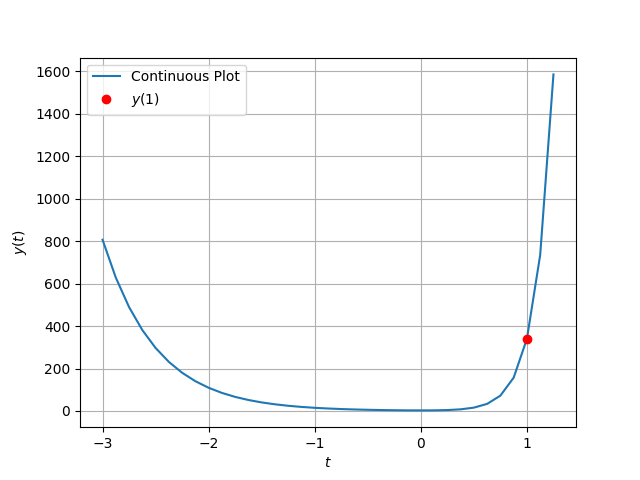
\includegraphics[width=\columnwidth]{2022/NM/50/figs/g50fig1.png}
    \caption{}    
    \label{fig:ishitha.g22.nm.50.f2}
\end{figure}
%\end{document}

\pagebreak

\item The Bode magnitude plot of a first order stable system is constant with frequency. The asymptotic value of the high frequency phase, for the system, is $-180\degree$ . This system has \\
\begin{figure}[h]
    \centering
    \resizebox{0.55\columnwidth}{!}{\begin{tikzpicture}[scale=1.5]
    % X-axis
    \draw[->] (0,0) -- (4,0) node[below] {$\log(f)$};
    % Y-axis
    \draw[<->] (0,-2) -- (0,2) node[left] {};
    % Y-axis labels
    \draw (0,-1) node[left] {$-180^\circ$};
    \draw (0,0) node[left] {$0^\circ$};
    % Straight line
    \draw (0,1) -- (3,1) node[right] {Magnitude};
   % Draw a curved line from (0,0) to (1,-1)
  \draw (0,0) to[out=-10, in=180] (1,-1);
 % Straight line
    \draw (1,-1) -- (3,-1) node[right] {Phase};
    \draw[dashed] (0,-1) -- (1,-1);
\end{tikzpicture}
}
    \caption{}
    \label{fig:gate2022ee17fig1}
\end{figure} \\
\begin{enumerate}[label={(\Alph*)}]
     \item one LHP pole and one RHP zero at the same frequency.
     \item one LHP pole and one LHP zero at the same frequency.
     \item two LHP poles and one RHP zero.
     \item two RHP poles and one LHP zero.
\end{enumerate}\hfill Gate 2022 EE 17 \\
\solution
\iffalse
\let\negmedspace\undefined
\let\negthickspace\undefined
\documentclass[journal,12pt,onecolumn]{IEEEtran}
\usepackage{cite}
\usepackage{amsmath,amssymb,amsfonts,amsthm}
\usepackage{algorithmic}
\usepackage{graphicx}
\usepackage{textcomp}
\usepackage{tikz}
\usepackage{xcolor}
\usepackage{txfonts}
\usepackage{listings}
\usepackage{pgfplots}
\usepackage{enumitem}
\usepackage{mathtools}
\usepackage{gensymb}

\usepackage{tkz-euclide} % loads  TikZ and tkz-base
\usepackage{listings}



\newtheorem{theorem}{Theorem}[section]
\newtheorem{problem}{Problem}
\newtheorem{proposition}{Proposition}[section]
\newtheorem{lemma}{Lemma}[section]
\newtheorem{corollary}[theorem]{Corollary}
\newtheorem{example}{Example}[section]
\newtheorem{definition}[problem]{Definition}
%\newtheorem{thm}{Theorem}[section] 
%\newtheorem{defn}[thm]{Definition}
%\newtheorem{algorithm}{Algorithm}[section]
%\newtheorem{cor}{Corollary}
\newcommand{\BEQA}{\begin{eqnarray}}
\newcommand{\EEQA}{\end{eqnarray}}
\newcommand{\system}[1]{\stackrel{#1}{\rightarrow}}

\newcommand{\define}{\stackrel{\triangle}{=}}
\theoremstyle{remark}
\newtheorem{rem}{Remark}
%\bibliographystyle{ieeetr}
\begin{document}
%
\providecommand{\pr}[1]{\ensuremath{\Pr\left(#1\right)}}
\providecommand{\prt}[2]{\ensuremath{p_{#1}^{\left(#2\right)} }}        % own macro for this question
\providecommand{\qfunc}[1]{\ensuremath{Q\left(#1\right)}}
\providecommand{\sbrak}[1]{\ensuremath{{}\left[#1\right]}}
\providecommand{\lsbrak}[1]{\ensuremath{{}\left[#1\right.}}
\providecommand{\rsbrak}[1]{\ensuremath{{}\left.#1\right]}}
\providecommand{\brak}[1]{\ensuremath{\left(#1\right)}}
\providecommand{\lbrak}[1]{\ensuremath{\left(#1\right.}}
\providecommand{\rbrak}[1]{\ensuremath{\left.#1\right)}}
\providecommand{\cbrak}[1]{\ensuremath{\left\{#1\right\}}}
\providecommand{\lcbrak}[1]{\ensuremath{\left\{#1\right.}}
\providecommand{\rcbrak}[1]{\ensuremath{\left.#1\right\}}}
\newcommand{\sgn}{\mathop{\mathrm{sgn}}}
\providecommand{\abs}[1]{\left\vert#1\right\vert}
\providecommand{\res}[1]{\Res\displaylimits_{#1}} 
\providecommand{\norm}[1]{\left\lVert#1\right\rVert}
%\providecommand{\norm}[1]{\lVert#1\rVert}
\providecommand{\mtx}[1]{\mathbf{#1}}
\providecommand{\mean}[1]{E\left[ #1 \right]}
\providecommand{\cond}[2]{#1\middle|#2}
\providecommand{\fourier}{\overset{\mathcal{F}}{ \rightleftharpoons}}
\newenvironment{amatrix}[1]{%
  \left(\begin{array}{@{}*{#1}{c}|c@{}}
}{%
  \end{array}\right)
}
%\providecommand{\hilbert}{\overset{\mathcal{H}}{ \rightleftharpoons}}
%\providecommand{\system}{\overset{\mathcal{H}}{ \longleftrightarrow}}
	%\newcommand{\solution}[2]{\textbf{Solution:}{#1}}
\newcommand{\solution}{\noindent \textbf{Solution: }}
\newcommand{\cosec}{\,\text{cosec}\,}
\providecommand{\dec}[2]{\ensuremath{\overset{#1}{\underset{#2}{\gtrless}}}}
\newcommand{\myvec}[1]{\ensuremath{\begin{pmatrix}#1\end{pmatrix}}}
\newcommand{\mydet}[1]{\ensuremath{\begin{vmatrix}#1\end{vmatrix}}}
\newcommand{\myaugvec}[2]{\ensuremath{\begin{amatrix}{#1}#2\end{amatrix}}}
\providecommand{\rank}{\text{rank}}
\providecommand{\pr}[1]{\ensuremath{\Pr\left(#1\right)}}
\providecommand{\qfunc}[1]{\ensuremath{Q\left(#1\right)}}
	\newcommand*{\permcomb}[4][0mu]{{{}^{#3}\mkern#1#2_{#4}}}
\newcommand*{\perm}[1][-3mu]{\permcomb[#1]{P}}
\newcommand*{\comb}[1][-1mu]{\permcomb[#1]{C}}
\providecommand{\qfunc}[1]{\ensuremath{Q\left(#1\right)}}
\providecommand{\gauss}[2]{\mathcal{N}\ensuremath{\left(#1,#2\right)}}
\providecommand{\diff}[2]{\ensuremath{\frac{d{#1}}{d{#2}}}}
\providecommand{\myceil}[1]{\left \lceil #1 \right \rceil }
\newcommand\figref{Fig.~\ref}
\newcommand\tabref{Table~\ref}
\newcommand{\sinc}{\,\text{sinc}\,}
\newcommand{\rect}{\,\text{rect}\,}
%%
%	%\newcommand{\solution}[2]{\textbf{Solution:}{#1}}
%\newcommand{\solution}{\noindent \textbf{Solution: }}
%\newcommand{\cosec}{\,\text{cosec}\,}
%\numberwithin{equation}{section}
%\numberwithin{equation}{subsection}
%\numberwithin{problem}{section}
%\numberwithin{definition}{section}
%\makeatletter
%\@addtoreset{figure}{problem}
%\makeatother

%\let\StandardTheFigure\thefigure
\let\vec\mathbf

\bibliographystyle{IEEEtran}





\bigskip


\title{Gate 2022\_EE\_17}
\author{Karyampudi Meghana Sai\\ EE23BTECH11031}

\maketitle

The Bode magnitude plot of a first order stable system is constant with frequency. The asymptotic value of the high frequency phase, for the system, is $-180\degree$ . This system has \\
\begin{figure}[h]
    \centering
    \resizebox{0.55\columnwidth}{!}{\begin{tikzpicture}[scale=1.5]
    % X-axis
    \draw[->] (0,0) -- (4,0) node[below] {$\log(f)$};
    % Y-axis
    \draw[<->] (0,-2) -- (0,2) node[left] {};
    % Y-axis labels
    \draw (0,-1) node[left] {$-180^\circ$};
    \draw (0,0) node[left] {$0^\circ$};
    % Straight line
    \draw (0,1) -- (3,1) node[right] {Magnitude};
   % Draw a curved line from (0,0) to (1,-1)
  \draw (0,0) to[out=-10, in=180] (1,-1);
 % Straight line
    \draw (1,-1) -- (3,-1) node[right] {Phase};
    \draw[dashed] (0,-1) -- (1,-1);
\end{tikzpicture}
}
    \caption{}
    \label{fig:gate2022ee17fig1}
\end{figure} \\
(A) one LHP pole and one RHP zero at the same frequency.\\
(B) one LHP pole and one LHP zero at the same frequency.\\
(C) two LHP poles and one RHP zero.\\
(D) two RHP poles and one LHP zero.\\
\hfill Gate 2022 EE 17

\solution\\
\fi
Flat constant magnitude response for all frequency of system shows that it is an all pass system.\\
In all pass system, poles and zeros are symmetrical about $j\omega$ axis.\\
Possible transfer functions are\\
\begin{align}
T_1 (s)&=\frac{s-a}{s+a} \quad a>0 \label{eq:gate2022eee17eq1}\\
T_2 (s)&=\frac{a-s}{a+s} \quad a>0 \label{eq:gate2022eee17eq2}\\
s&=j\omega\label{eq:gate2022eee17eq3}
\end{align}
From the phase plot as $\omega \system{} \infty$ shows $\phi= -180\degree$.\\
\begin{enumerate}
\item For $T_1(s)$:\\
Using equation \eqref{eq:gate2022eee17eq3}\\
\begin{align}
T_1 (j \omega)&=\frac{j \omega -a}{j \omega +a} \quad a>0 \\
\angle T_1(j\omega)&=180\degree - \tan^{-1}\brak{\frac{\omega}{a}}-\tan^{-1}\brak{\frac{\omega}{a}}\\
&=180\degree - 2\tan^{-1}\brak{\frac{\omega}{a}}
\end{align}
At $\omega=\infty$,
\begin{align}
\angle T_1(j\omega)=0\degree
\end{align}
\item For $T_2(s)$:\\
Using equation \eqref{eq:gate2022eee17eq3}\\
\begin{align}
T_2 (j \omega)&=\frac{a-j \omega }{a+j \omega} \quad a>0 \\
\angle T_2(j\omega)&=- \tan^{-1}\brak{\frac{\omega}{a}}-\tan^{-1}\brak{\frac{\omega}{a}}\\
&=- 2\tan^{-1}\brak{\frac{\omega}{a}}
\end{align}
At $\omega=\infty$,
\begin{align}
\angle T_2(j\omega)=-180\degree
\end{align}
\end{enumerate}
Hence, the transfer function of given all pass filter.\\
\begin{align}
T(s)=\frac{a-s}{a+s} \quad a>0
\end{align}
Hence, the system has one LHP pole and one RHP zero at the same frequency.
%\end{document}

\newpage

\end{enumerate}
